\chapter{控制方程}
\section{纳维-斯托克斯方程}
%\subsection{模型}
\subsection{连续性微分方程}
连续性微分方程是质量守恒定律在流场中固定的无穷小微元控制体所导出的,即单位时间内
净流入控制体内的质量等于单位时间内控制体内质量的增加量。如图\ref{FgCGe_Ce}所示,任取
一固定在流场中的无穷小正交六面体控制体,各边分别与直角坐标系各轴平行,各边边长分别为$\mathrm{d}x$、
$\mathrm{d}y$和$\mathrm{d}z$。控制体中心坐标为$(x,y,z)$,密度为$\rho$
,速度为$(u,v,w)$。$\rho$、$u$、$v$和$w$均为$x,y,z,t$的函数。
\begin{figure}[h]
  \centering
  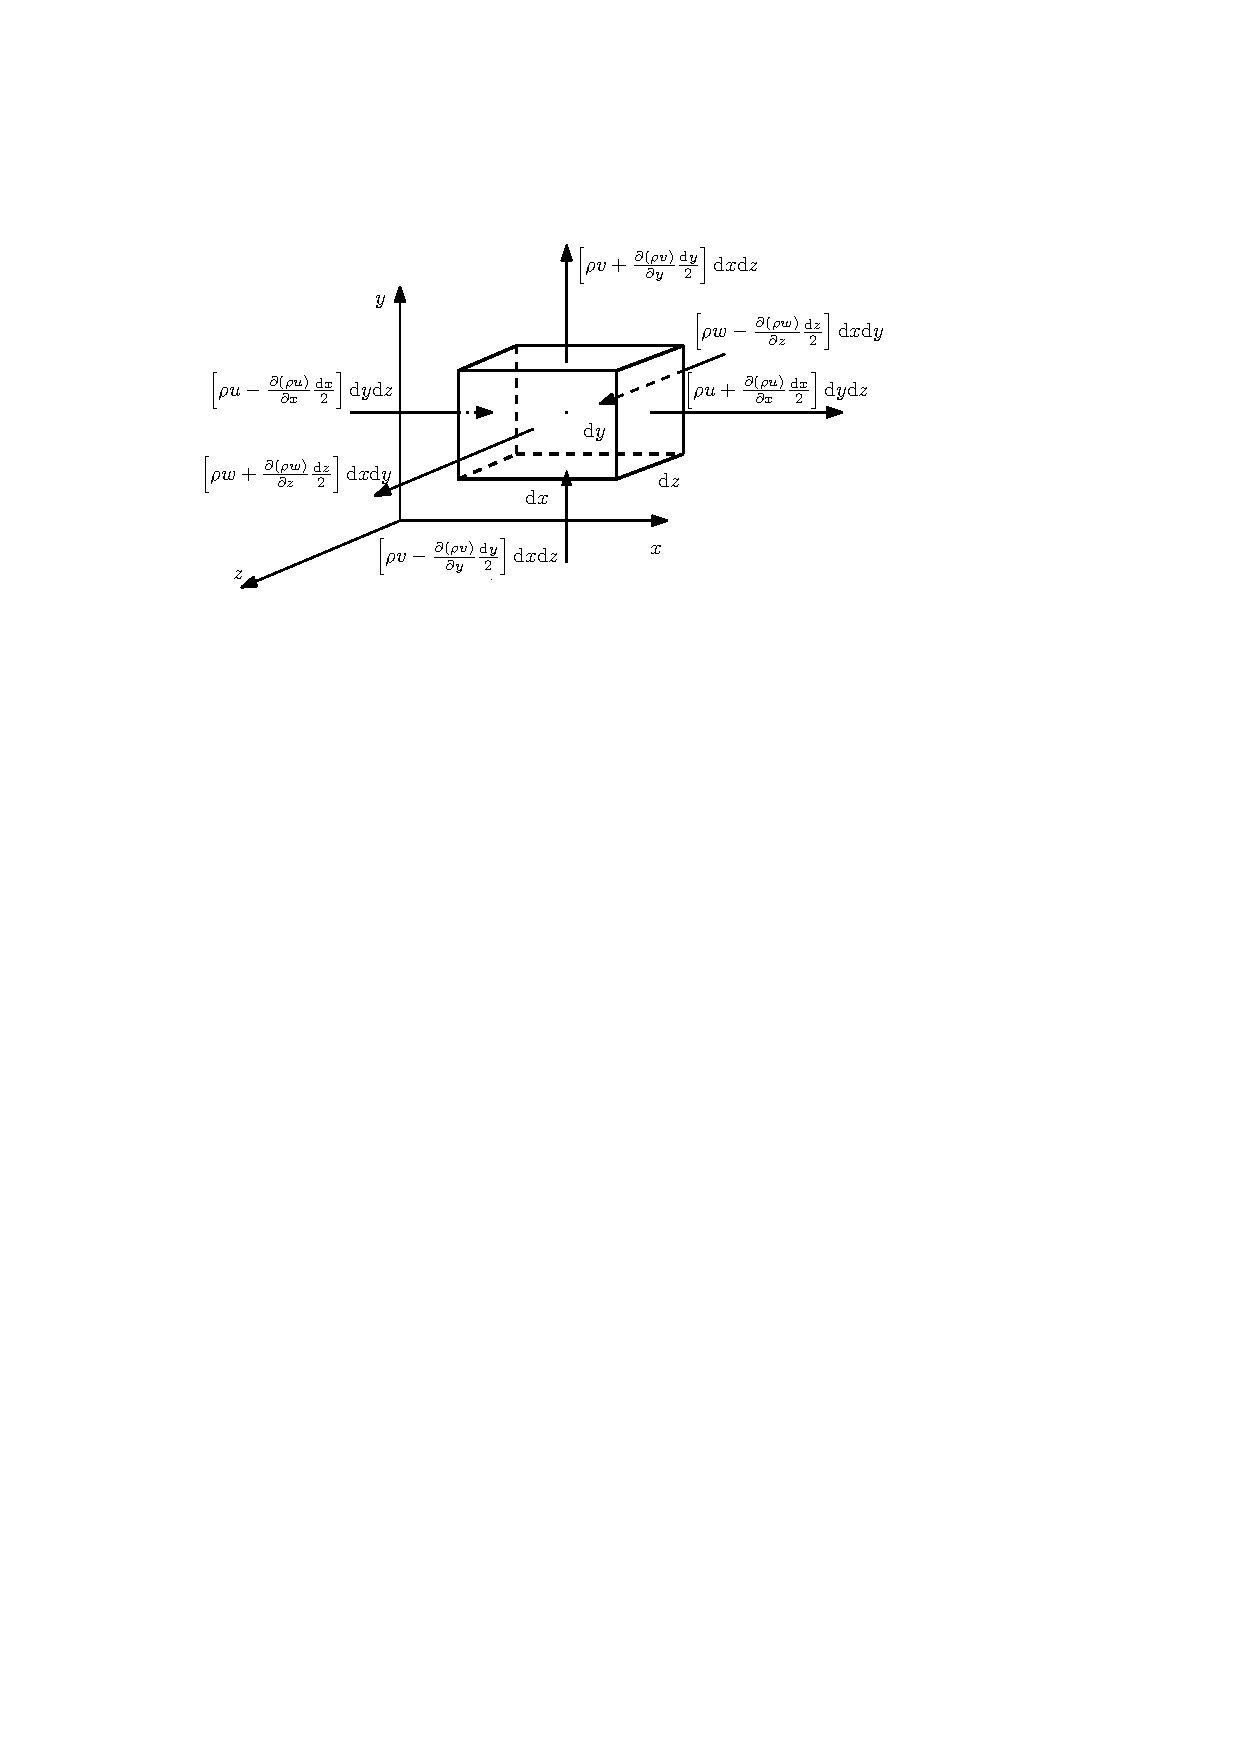
\includegraphics{CGeCe.pdf}
  \caption{固定在流场中的无穷小正交六面体控制体和质量流量示意图}
  \label{FgCGe_Ce}
\end{figure}

流体可以穿过外表面流入或流出控制体。
以$x$方向为例,流体从控制体的左侧和右侧两个面进出控制体。根据泰勒展开并略去高阶无穷小量,单位时间内从左侧面流入
控制体的质量为
\begin{equation*}
  \left[\rho u-\frac{\partial (\rho u)}{\partial x}\frac {\mathrm{d}x}{2}\right]\mathrm{d}y\mathrm{d}z
\end{equation*}
单位时间内从右侧面流出控制体的质量为
\begin{equation*}
  \left[\rho u+\frac{\partial (\rho u)}{\partial x}\frac {\mathrm{d}x}{2}\right]\mathrm{d}y\mathrm{d}z
\end{equation*}
因此,单位时间沿$x$方向净流入控制体的质量为
\begin{equation}
  -\frac{\partial (\rho u)}{\partial x}\mathrm{d}x\mathrm{d}y\mathrm{d}z
\end{equation}
同理,单位时间内沿$y$、$z$方向净流入控制体的质量分别为
\begin{equation*}
  -\frac{\partial (\rho v)}{\partial y}\mathrm{d}x\mathrm{d}y\mathrm{d}z
  \mbox{和}
  -\frac{\partial (\rho w)}{\partial z}\mathrm{d}x\mathrm{d}y\mathrm{d}z
\end{equation*}
因此,单位时间内净流入控制体内的质量为
\begin{equation}
  -\left[
    \frac {\partial (\rho u)} {\partial x}
    +
    \frac {\partial (\rho v)} {\partial y}
    +
    \frac {\partial (\rho w)} {\partial z}
    \right]
    \mathrm{d}x\mathrm{d}y\mathrm{d}z
\end{equation}

控制体的质量为$\rho\mathrm{d}x\mathrm{d}y\mathrm{d}z$,单位时间内控制体内质量的增加量为
\begin{equation}
  \frac{\partial}{\partial t}(\rho\mathrm{d}x\mathrm{d}y\mathrm{d}z) =
  \frac{\partial \rho}{\partial  t}\mathrm{d}x\mathrm{d}y\mathrm{d}z
\end{equation}

根据质量守恒定律,有
\begin{equation}
  \frac{\partial \rho}{\partial  t}\mathrm{d}x\mathrm{d}y\mathrm{d}z
  =
  -
  \left[
    \frac {\partial (\rho u)} {\partial x}
    +
    \frac {\partial (\rho v)} {\partial y}
    +
    \frac {\partial (\rho w)} {\partial z}
    \right]
    \mathrm{d}x\mathrm{d}y\mathrm{d}z
\end{equation}
上式两边同除以$\mathrm{d}x\mathrm{d}y\mathrm{d}z$后,将等号右边所有项移到左边,即得连续性
微分方程
\begin{equation}
  \frac{\partial \rho}{\partial  t}
  +
  \frac{\partial (\rho u)}{\partial  x}
  +
  \frac{\partial (\rho v)}{\partial  y}
  +
  \frac{\partial (\rho w)}{\partial  z}
  =
  0
\end{equation}
对均质不可压缩流体,$\rho$为常数,连续性方程可写成
\begin{equation}
  \frac{\partial u}{\partial  x}
  +
  \frac{\partial v}{\partial  y}
  +
  \frac{\partial w}{\partial  z}
  =
  0
  \label{EqCGe_NS_Ce}
\end{equation}

\subsection{动量方程}
动量方程是牛顿第二定律或动量守恒定律得数学表达式。如图\ref{FgCGe_Me}所示,考虑一
个随流运动的无穷小正交六面体流体微团。微团中心点所在坐标为$(x,y,z)$,中心点密度
为$\rho$,速度为$(u, v, w)$,压强为$p$。则该微团的质量
为
\begin{equation}
  m = \rho\mathrm{d}x\mathrm{d}y\mathrm{d}z
\end{equation}

\begin{figure}[hb]
  \centering
  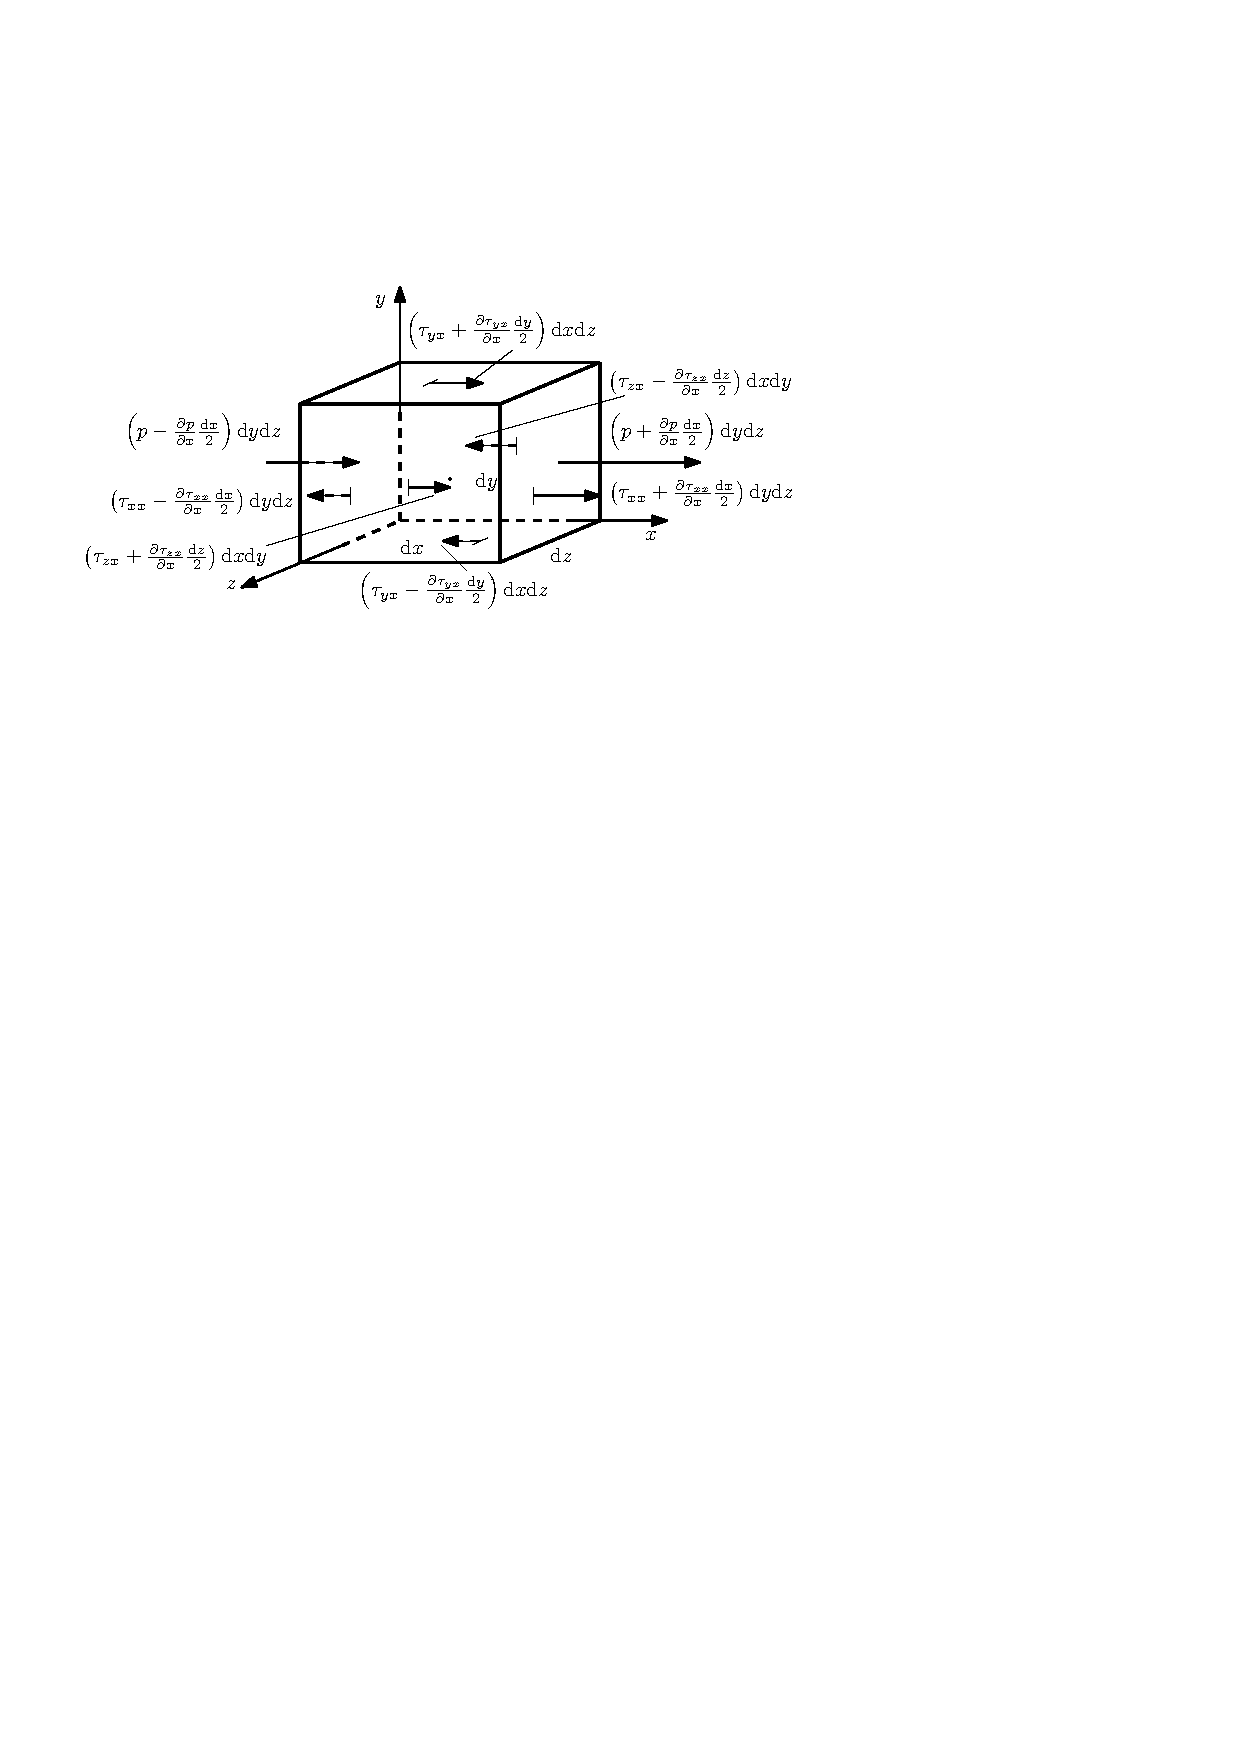
\includegraphics{CGeMe.pdf}
  \caption{随流运动的流体微团在$x$方向表面力受力分析}
  \label{FgCGe_Me}
\end{figure}

$x$方向的牛顿第二定律为
\begin{equation}
  F_{x} = ma_{x}
  \label{EqCGe_Nt_x}
\end{equation}
式中,$F_{x}$和$a_{x}$分别是微团所受外力和加速度在$x$方向的分量。

随流运动的流体微团的$a_{x}$等于$u_{x}$随时间的变化率,即速度的
随体导数
\begin{equation}
  a_{x} =
  \frac{\mathrm{D}u}{\mathrm{D}t}
  \label{EqCGe_Ac_x}
\end{equation}

流体微团在$x$方向所受外力有两类:体积力$F_{x}$和表面力$T_{x}$。假定作用在微团上的单位质量力为
$\mathbf{f}=(f_{x}, f_{y}, f_{z})$。$x$方向所受的体积力为:
\begin{equation}
  F_{x} = \rho f_{x}\mathrm{d}x\mathrm{d}y\mathrm{d}z
  \label{EqCGe_Bf_x}
\end{equation}
如图\ref{FgCGe_Me}所示,表面力$T_{x}$是直接作用在六个外表面上的力,包括:(1)作用在外表面上的压力;(2)作用在
外表面上正压力和剪切力。在$x$方向上,只有左侧面和右侧面的压力,分别为
$(p-\frac{\partial p}{\partial x}\frac{\mathrm{d}x}{2})\mathrm{d}y\mathrm{d}z$和
$-(p+\frac{\partial p}{\partial x}\frac{\mathrm{d}x}{2})\mathrm{d}y\mathrm{d}z$
。作用在
六个外表面上在$x$方向上的正应力和切应力共6个,即
左侧面上的
$-(\tau_{xx}-\frac{\partial \tau_{xx}}{\partial x}\frac{\mathrm{d}x}{2})\mathrm{d}y\mathrm{d}z$,
右侧面上的
$(\tau_{xx}+\frac{\partial \tau_{xx}}{\partial x}\frac{\mathrm{d}x}{2})\mathrm{d}y\mathrm{d}z$,
前侧面上的
$(\tau_{zx}+\frac{\partial \tau_{zx}}{\partial z}\frac{\mathrm{d}z}{2})\mathrm{d}x\mathrm{d}y$,
后侧面上的
$-(\tau_{zx}-\frac{\partial \tau_{zx}}{\partial z}\frac{\mathrm{d}z}{2})\mathrm{d}x\mathrm{d}y$,
底侧面上的
$-(\tau_{yx}-\frac{\partial \tau_{yx}}{\partial y}\frac{\mathrm{d}y}{2})\mathrm{d}x\mathrm{d}z$,
顶侧面上的
$(\tau_{yx}+\frac{\partial \tau_{yx}}{\partial y}\frac{\mathrm{d}y}{2})\mathrm{d}x\mathrm{d}z$,
上述应力表述中,下标第一项表示该作用面的法向方向,第二项表示应力的正向方向,正负
号表示力的方向。
\begin{equation}
  \begin{aligned}
    T_{x} =&
    \left[
      \left(p-\frac{\partial p}{\partial x}\frac{\mathrm{d}x}{2}\right)
      -
      \left(p+\frac{\partial p}{\partial x}\frac{\mathrm{d}x}{2}\right)
    \right]\mathrm{d}y\mathrm{d}z 
    +
    \\
    &
    \left[
      \left(\tau_{xx}+\frac{\partial \tau_{xx}}{\partial x}\frac{\mathrm{d}x}{2}\right)
      -
      \left(\tau_{xx}-\frac{\partial \tau_{xx}}{\partial x}\frac{\mathrm{d}x}{2}\right)
    \right]
    \mathrm{d}y\mathrm{d}z +\\
    & 
    \left[
      \left(\tau_{yx}+\frac{\partial \tau_{yx}}{\partial y}\frac{\mathrm{d}y}{2}\right)
      -
      \left(\tau_{yx}-\frac{\partial \tau_{yx}}{\partial y}\frac{\mathrm{d}y}{2}\right)
    \right]
    \mathrm{d}x\mathrm{d}z
    + \\
    &\left[
      \left(\tau_{zx}+\frac{\partial \tau_{zx}}{\partial z}\frac{\mathrm{d}z}{2}\right)
      -
      \left(\tau_{zx}-\frac{\partial \tau_{zx}}{\partial z}\frac{\mathrm{d}z}{2}\right)
    \right]
    \mathrm{d}x\mathrm{d}y
    \\
    =&
    \left(
    -\frac{\partial p}{\partial x}
    +\frac{\partial \tau_{xx}}{\partial x}
    +\frac{\partial \tau_{yx}}{\partial y}
    +\frac{\partial \tau_{zx}}{\partial z}
    \right)
    \mathrm{d}x\mathrm{d}y\mathrm{d}z
  \end{aligned}
  \label{EqCGe_Sf_x}
\end{equation}
将式\eqref{EqCGe_Ac_x}、\eqref{EqCGe_Bf_x}和\eqref{EqCGe_Sf_x}代入式
\eqref{EqCGe_Nt_x},可得到$x$方向的动量方程。同理可得,$y$和$z$方向的动量方程。
最终得到的动量方程为
\begin{equation}
  \begin{aligned}
    \rho \frac{\mathrm{D}u}{\mathrm{D}t} =
    \rho f_{x}
    -\frac{\partial p}{\partial x}
    +\frac{\partial \tau_{xx}}{\partial x}
    +\frac{\partial \tau_{yx}}{\partial y}
    +\frac{\partial \tau_{zx}}{\partial z}
    \\
    \rho \frac{\mathrm{D}v}{\mathrm{D}t} =
    \rho f_{y}
    -\frac{\partial p}{\partial y}
    +\frac{\partial \tau_{xy}}{\partial x}
    +\frac{\partial \tau_{yy}}{\partial y}
    +\frac{\partial \tau_{zy}}{\partial z}
    \\
    \rho \frac{\mathrm{D}w}{\mathrm{D}t} =
    \rho f_{z}
    -\frac{\partial p}{\partial z}
    +\frac{\partial \tau_{xz}}{\partial x}
    +\frac{\partial \tau_{yz}}{\partial y}
    +\frac{\partial \tau_{zz}}{\partial z}
  \end{aligned}
  \label{EqCGe_NS_Me_ori}
\end{equation}

根据数学知识,
\begin{equation}
  \begin{aligned}
    \rho \frac{\mathrm{D}u}{\mathrm{D}t}
    =
    \frac{\partial (\rho u)}{\partial t}
    +
    \nabla\cdot(\rho u\mathbf{u})
    =
    \frac{\partial (\rho u)}{\partial t}
    +
    \frac{\partial \rho (uu)}{\partial x}
    +
    \frac{\partial \rho (uv)}{\partial y}
    +
    \frac{\partial \rho (uw)}{\partial z}
    \\
    \rho \frac{\mathrm{D}v}{\mathrm{D}t}
    =
    \frac{\partial (\rho v)}{\partial t}
    +
    \nabla\cdot(\rho v\mathbf{u})
    =
    \frac{\partial (\rho v)}{\partial t}
    +
    \frac{\partial \rho (vu)}{\partial x}
    +
    \frac{\partial \rho (vv)}{\partial y}
    +
    \frac{\partial \rho (vw)}{\partial z}
    \\
    \rho \frac{\mathrm{D}w}{\mathrm{D}t}
    =
    \frac{\partial (\rho w)}{\partial t}
    +
    \nabla\cdot(\rho w\mathbf{u})
    =
    \frac{\partial (\rho w)}{\partial t}
    +
    \frac{\partial \rho (wu)}{\partial x}
    +
    \frac{\partial \rho (wv)}{\partial y}
    +
    \frac{\partial \rho (ww)}{\partial z}
  \end{aligned}
  \label{EqCGe_div}
\end{equation}
将式\eqref{EqCGe_div}代入式\eqref{EqCGe_NS_Me_ori}中,
\begin{equation}
  \begin{aligned}
    \frac{\partial (\rho u)}{\partial t}
    +
    \frac{\partial \rho (uu)}{\partial x}
    +
    \frac{\partial \rho (uv)}{\partial y}
    +
    \frac{\partial \rho (uw)}{\partial z}
    =
    \rho f_{x}
    -\frac{\partial p}{\partial x}
    +\frac{\partial \tau_{xx}}{\partial x}
    +\frac{\partial \tau_{yx}}{\partial y}
    +\frac{\partial \tau_{zx}}{\partial z}
    \\
    \frac{\partial (\rho v)}{\partial t}
    +
    \frac{\partial \rho (vu)}{\partial x}
    +
    \frac{\partial \rho (vv)}{\partial y}
    +
    \frac{\partial \rho (vw)}{\partial z}
    =
    \rho f_{y}
    -\frac{\partial p}{\partial y}
    +\frac{\partial \tau_{xy}}{\partial x}
    +\frac{\partial \tau_{yy}}{\partial y}
    +\frac{\partial \tau_{zy}}{\partial z}
    \\
    \frac{\partial (\rho w)}{\partial t}
    +
    \frac{\partial \rho (wu)}{\partial x}
    +
    \frac{\partial \rho (wv)}{\partial y}
    +
    \frac{\partial \rho (ww)}{\partial z}
    =
    \rho f_{z}
    -\frac{\partial p}{\partial z}
    +\frac{\partial \tau_{xz}}{\partial x}
    +\frac{\partial \tau_{yz}}{\partial y}
    +\frac{\partial \tau_{zz}}{\partial z}
  \end{aligned}
  \label{EqCGe_NS_Me_general}
\end{equation}

在17世纪晚期,牛顿给出了牛顿内摩擦定律,即流体内部切应力正比于剪切变形速率。1845
年,斯托克斯给出如下关系式
\begin{equation}
  \begin{aligned}
    &\tau_{xx} = \lambda(\nabla\cdot\mathbf{u}) + 2\mu\frac{\partial u}{\partial x}
    \\&
    \tau_{yy} = \lambda(\nabla\cdot\mathbf{u}) + 2\mu\frac{\partial v}{\partial y}
    \\&
    \tau_{zz} = \lambda(\nabla\cdot\mathbf{u}) + 2\mu\frac{\partial w}{\partial z}
    \\&
    \tau_{xy} = \tau_{yx} =
    \mu
    \left(
    \frac{\partial v}{\partial x}+\frac{\partial u}{\partial y}
    \right)
    \\&
    \tau_{xz} = \tau_{zx} =
    \mu
    \left(
    \frac{\partial u}{\partial z}+\frac{\partial w}{\partial x}
    \right)
    \\&
    \tau_{yz} = \tau_{zy} =
    \mu
    \left(
    \frac{\partial w}{\partial y}+\frac{\partial v}{\partial z}
    \right)
  \end{aligned}
  \label{EqCGe_Stokes}
\end{equation}
式中,$\mu$为流体动力粘滞系数,$\lambda$是第二粘滞系数。斯托克斯假定
\begin{equation}
  \lambda = -\frac{2}{3}\mu
  \label{EqCGe_Stokes_labmda}
\end{equation}
将式\eqref{EqCGe_Stokes}和\eqref{EqCGe_Stokes_labmda}代入式
\eqref{EqCGe_NS_Me_general},得
\begin{subequations}
  \begin{align}
    \begin{aligned}
      \frac{\partial (\rho u)}{\partial t}
      +&
      \frac{\partial \rho (uu)}{\partial x}
      +
      \frac{\partial \rho (uv)}{\partial y}
      +
      \frac{\partial \rho (uw)}{\partial z}
      =
      \rho f_{x}
      -\frac{\partial p}{\partial x} \\
      &+\frac{\partial }{\partial x}
      \left[
        \lambda(\nabla\cdot\mathbf{u}) + 2\mu\frac{\partial u}{\partial x}
      \right]
      +\frac{\partial }{\partial y}
      \left[
        \mu
        \left(
        \frac{\partial v}{\partial x}+\frac{\partial u}{\partial y}
        \right)
      \right]
      +\frac{\partial }{\partial z}
      \left[
        \mu
        \left(
        \frac{\partial u}{\partial z}+\frac{\partial w}{\partial x}
        \right)
      \right]
    \end{aligned}
    \label{EqCGe_NS_Me_general_expand_1}
    \\
    \begin{aligned}
      \frac{\partial (\rho v)}{\partial t}
      +&
      \frac{\partial \rho (vu)}{\partial x}
      +
      \frac{\partial \rho (vv)}{\partial y}
      +
      \frac{\partial \rho (vw)}{\partial z}
      =
      \rho f_{y}
      -\frac{\partial p}{\partial y} \\
      &+\frac{\partial }{\partial x}
      \left[
        \mu
        \left(
        \frac{\partial v}{\partial x}+\frac{\partial u}{\partial y}
        \right)
      \right]
      +\frac{\partial }{\partial y}
      \left[
        \lambda(\nabla\cdot\mathbf{u}) + 2\mu\frac{\partial v}{\partial y}
      \right]
      +\frac{\partial }{\partial z}
      \left[
        \mu
        \left(
        \frac{\partial w}{\partial y}+\frac{\partial v}{\partial z}
        \right)
      \right]
    \end{aligned}
    \\
    \begin{aligned}
      \frac{\partial (\rho w)}{\partial t}
      &+
      \frac{\partial \rho (wu)}{\partial x}
      +
      \frac{\partial \rho (wv)}{\partial y}
      +
      \frac{\partial \rho (ww)}{\partial z}
      =
      \rho f_{z}
      -\frac{\partial p}{\partial z} \\
      &+\frac{\partial }{\partial x}
      \left[
        \mu
        \left(
        \frac{\partial u}{\partial z}+\frac{\partial w}{\partial x}
        \right)
      \right]
      +\frac{\partial }{\partial y}
      \left[
        \mu
        \left(
        \frac{\partial w}{\partial y}+\frac{\partial v}{\partial z}
        \right)
      \right]
      +\frac{\partial }{\partial z}
      \left[
        \lambda(\nabla\cdot\mathbf{u}) + 2\mu\frac{\partial w}{\partial z}
      \right]
    \end{aligned}
  \end{align}
  \label{EqCGe_NS_Me_general_expand}
\end{subequations}
式\eqref{EqCGe_NS_Me_general_expand_1}中第二行的各项可以进一步展开为
\begin{equation}
  \begin{aligned}
    &\frac{\partial }{\partial x}
    \left[
      \lambda(\nabla\cdot\mathbf{u}) + 2\mu\frac{\partial u}{\partial x}
    \right]
    +\frac{\partial }{\partial y}
    \left[
      \mu
      \left(
      \frac{\partial v}{\partial x}+\frac{\partial u}{\partial y}
      \right)
    \right]
    +\frac{\partial }{\partial z}
    \left[
      \mu
      \left(
      \frac{\partial u}{\partial z}+\frac{\partial w}{\partial x}
      \right)
    \right]
    \\
    &=
    \mu
    \left(
    \frac{\partial^{2} u}{\partial x^{2}} +
    \frac{\partial^{2} u}{\partial y^{2}} +
    \frac{\partial^{2} u}{\partial z^{2}}
    \right)
    +
    \mu
    \frac{\partial}{\partial x}
    \left(
    \frac{\partial u}{\partial x} +
    \frac{\partial v}{\partial y} +
    \frac{\partial w}{\partial z}
    \right)
    +
    \frac{\partial}{\partial x}[\lambda(\nabla\cdot\mathbf{u})]
    \\
    &=
    \mu
    \left(
    \frac{\partial^{2} u}{\partial x^{2}} +
    \frac{\partial^{2} u}{\partial y^{2}} +
    \frac{\partial^{2} u}{\partial z^{2}}
    \right)
    +
    \mu
    \frac{\partial}{\partial x}
    \left(
    \nabla\cdot\mathbf{u}
    \right)
    +
    \frac{\partial}{\partial x}[\lambda(\nabla\cdot\mathbf{u})]
  \end{aligned}
\end{equation}
对均质不可压缩流体,其连续性方程为$\nabla\cdot\mathbf{u}=0$,上式最后得到
\begin{equation}
  \mu
  \left(
  \frac{\partial^{2} u}{\partial x^{2}} +
  \frac{\partial^{2} u}{\partial y^{2}} +
  \frac{\partial^{2} u}{\partial z^{2}}
  \right)
\end{equation}
对\eqref{EqCGe_NS_Me_general_expand}的后两个公式采用同样的处理方式,并代入均质不
可压缩条件,式\eqref{EqCGe_NS_Me_general_expand}可以写成
\begin{subequations}
  \begin{align}
    \frac{\partial u}{\partial t}
    +
    \frac{\partial (uu)}{\partial x}
    +
    \frac{\partial (uv)}{\partial y}
    +
    \frac{\partial (uw)}{\partial z}
    =
    f_{x}
    -\frac{1}{\rho}\frac{\partial p}{\partial x}
    +
    \nu
    \left(
    \frac{\partial^{2} u}{\partial x^{2}} +
    \frac{\partial^{2} u}{\partial y^{2}} +
    \frac{\partial^{2} u}{\partial z^{2}}
    \right)
    \label{EqCGe_NS_Me_x}
    \\
    \frac{\partial v}{\partial t}
    +
    \frac{\partial (vu)}{\partial x}
    +
    \frac{\partial (vv)}{\partial y}
    +
    \frac{\partial (vw)}{\partial z}
    =
    f_{y}
    -\frac{1}{\rho}\frac{\partial p}{\partial y}
    +
    \nu
    \left(
    \frac{\partial^{2} v}{\partial x^{2}} +
    \frac{\partial^{2} v}{\partial y^{2}} +
    \frac{\partial^{2} v}{\partial z^{2}}
    \right)
    \\
    \frac{\partial w}{\partial t}
    +
    \frac{\partial (wu)}{\partial x}
    +
    \frac{\partial (wv)}{\partial y}
    +
    \frac{\partial (ww)}{\partial z}
    =
    f_{z}
    -\frac{1}{\rho}\frac{\partial p}{\partial z}
    +
    \nu
    \left(
    \frac{\partial^{2} w}{\partial x^{2}} +
    \frac{\partial^{2} w}{\partial y^{2}} +
    \frac{\partial^{2} w}{\partial z^{2}}
    \right)
  \end{align}
  \label{EqCGe_NS_Me}
\end{subequations}
或写成矢量形式为
\begin{equation}
  \frac{\partial \mathbf{u}}{\partial x} +
  \nabla\cdot(\mathbf{u}\mathbf{u})
  =
  \mathbf{f} -
  \frac{1}{\rho}\nabla p +
  \nu\nabla^{2}\mathbf{u}
\end{equation}


\section{雷诺时均方程}
\subsection{紊流物理量时均值定义及性质}
根据大量相关实验观测,紊流具有有涡性、不规则性、耗能性、连续性、三维性以及非定常
性等特征。因此,紊流运动要素都具有随机性。为了分析方便,紊流运动要素的瞬时值
常被分解成时均值和脉动值。任一运动要素$\phi$的时均值定义为:
\begin{equation}
  \overline{\phi}
  =
  \frac{1}{\Delta t}
  \int_{t}^{t+\Delta t}\!
  \phi(t)
  \mathrm{d}t
  \label{EqCGe_RA}
\end{equation}
其中,时间间隔$\Delta t$相对于紊流的随机脉动周期而言足够大,但相对于流场的各种时
均量的缓慢变化周期来说,应足够小。如果时均值随时间变化,成为非稳态的时均紊流;如
果时均值不随时间变化,成为准稳态紊流,简称稳态紊流。


运动要素的瞬时值$\phi$,时均值$\overline{\phi}$及脉动值$\phi^{\prime}$之间有如下
关系:
\begin{equation}
  \phi = \overline{\phi} + \phi^{\prime}
  \label{EqCGe_RA_Comp}
\end{equation}

设$\phi$和$f$是两个瞬时值,$\overline{\phi}$和$\overline{f}$为相应的时均值,
$\phi^{\prime}$和$f^{\prime}$为相应的脉动值。按照式\eqref{EqCGe_RA}和
\eqref{EqCGe_RA_Comp},下列基本关系成立:
\begin{equation}
  \begin{aligned}
    &\overline{\phi^{\prime}} = 0
    \quad\quad
    \overline{\overline{\phi}} = \overline{\phi}
    \quad\quad
    \overline{\overline{\phi}+\phi^{\prime}} = \overline{\phi}
    \\
    & \overline{\overline{\phi}f} = \overline{\phi}\overline{f}
    \quad\quad
    \overline{\widebar{\phi}\widebar{f}} = \overline{\phi}\overline{f}
    \quad\quad
    \overline{\overline{\phi}f^{\prime}} = 0
    \quad\quad
    \overline{\phi f} = \widebar{\phi}\widebar{f} +
    \overline{\phi^{\prime}f^{\prime}}
    \\
    & \overline{\frac{\partial\phi}{\partial x_{i}}} = \frac{\partial \overline{\phi}}{\partial x_{i}}
    \quad\quad
    \overline{\frac{\partial^{2}\phi}{\partial x_{i}^{2}}} = \frac{\partial^{2}
    \overline{\phi}}{\partial x_{i}^{2}}
    \quad\quad
    \overline{\frac{\partial\phi^{\prime}}{\partial x_{i}}} = 0
    \quad\quad
    \overline{\frac{\partial^{2}\phi^{\prime}}{\partial x_{i}^{2}}} = 0
  \end{aligned}
  \label{EqCGe_RA_cal}
\end{equation}

\subsection{雷诺时均连续性方程}
将$u$、$v$和$w$表示成时均值和脉动值之和,并带入连续性方程\eqref{EqCGe_NS_Ce},并做时均运算
,
\begin{equation*}
  \overline{
    \frac{\partial(\overline{u}+u^{\prime})}{\partial x}
  }
  +
  \overline{
    \frac{\partial(\overline{v}+v^{\prime})}{\partial y}
  }
  +
  \overline{
    \frac{\partial(\overline{w}+w^{\prime})}{\partial z}
  }
  =
  \frac{\partial \overline{u}}{\partial x} +
  \frac{\partial \overline{v}}{\partial y} +
  \frac{\partial \overline{w}}{\partial z} +
  \frac{\partial \overline{u^{\prime}}}{\partial x} +
  \frac{\partial \overline{v^{\prime}}}{\partial y} +
  \frac{\partial \overline{w^{\prime}}}{\partial z}
  =0
\end{equation*}
运用式\eqref{EqCGe_RA_cal},可得
\begin{equation}
  \frac{\partial \overline{u}}{\partial x} +
  \frac{\partial \overline{v}}{\partial y} +
  \frac{\partial \overline{w}}{\partial z}
  =
  0
\end{equation}
上式表明,紊流速度的时均值仍满足连续性方程。

\subsection{雷诺时均运动方程}
以式\eqref{EqCGe_NS_Me_x}给出的$x$方向的运动方程为例,采取类似于连续性方程的处理,有
\begin{equation*}
  \begin{aligned}
    \overline{
      \frac{\partial (\overline{u}+u^{\prime})}{\partial t}
    }
    +
    \overline{
      \frac{\partial (\overline{u}+u^{\prime})^{2}}{\partial x}
    }
    +
    \overline{
      \frac{\partial (\overline{u}+u^{\prime})(\overline{v}+v^{\prime})}{\partial y}
    }
    +
    \overline{
      \frac{\partial (\overline{u}+u^{\prime})(\overline{w}+w^{\prime})}{\partial z}
    }
    \\
    =
    \overline{f_{x}}
    -\frac{1}{\rho}
    \overline{
      \frac{\partial (\overline{p}+p^{\prime})}{\partial x}
    }
    +
    \nu
    \left[
      \overline{
        \frac{\partial^{2} (\overline{u}+u^{\prime})}{\partial x^{2}}
      }
      +
      \overline{
        \frac{\partial^{2} (\overline{u}+u^{\prime})}{\partial y^{2}}
      }
      +
      \overline{
        \frac{\partial^{2} (\overline{u}+u^{\prime})}{\partial z^{2}}
      }
    \right]
  \end{aligned}
\end{equation*}
运用式\eqref{EqCGe_RA_cal},可得
\begin{equation*}
  \frac{\partial \overline{u}}{\partial t} +
  \frac{\partial \widebar{u}\widebar{u}}{\partial x} +
  \frac{\partial \widebar{u}\widebar{v}}{\partial y} +
  \frac{\partial \widebar{u}\widebar{w}}{\partial z} +
  \frac{\partial \overline{u^{\prime}u^{\prime}}}{\partial x} +
  \frac{\partial \overline{u^{\prime}v^{\prime}}}{\partial y} +
  \frac{\partial \overline{u^{\prime}w^{\prime}}}{\partial z}
  =
  \overline{f_{x}}
  -\frac{1}{\rho}\frac{\partial \overline{p}}{\partial x} +
  \nu
  \left(
  \frac{\partial^{2} \overline{u}}{\partial x^{2}} +
  \frac{\partial^{2} \overline{u}}{\partial y^{2}} +
  \frac{\partial^{2} \overline{u}}{\partial z^{2}}
  \right)
\end{equation*}
将上式左侧脉动值乘积的时均值移到等号右侧,得:
\begin{equation}
  \frac{\partial \overline{u}}{\partial t} +
  \frac{\partial \widebar{u}\widebar{u}}{\partial x} +
  \frac{\partial \widebar{u}\widebar{v}}{\partial y} +
  \frac{\partial \widebar{u}\widebar{w}}{\partial z}
  =
  \overline{f_{x}}
  -\frac{1}{\rho}\frac{\partial \overline{p}}{\partial x} -
  \left(
  \frac{\partial \overline{u^{\prime}u^{\prime}}}{\partial x} +
  \frac{\partial \overline{u^{\prime}v^{\prime}}}{\partial y} +
  \frac{\partial \overline{u^{\prime}w^{\prime}}}{\partial z}
  \right)
  +
  \nu
  \left(
  \frac{\partial^{2} \overline{u}}{\partial x^{2}} +
  \frac{\partial^{2} \overline{u}}{\partial y^{2}} +
  \frac{\partial^{2} \overline{u}}{\partial z^{2}}
  \right)
  \label{EqCGe_Ra_Me_temp1}
\end{equation}
同理可得,$y$和$z$方向的雷诺平均方程为:
\begin{equation}
  \frac{\partial \overline{v}}{\partial t} +
  \frac{\partial \widebar{v}\widebar{u}}{\partial x} +
  \frac{\partial \widebar{v}\widebar{v}}{\partial y} +
  \frac{\partial \widebar{v}\widebar{w}}{\partial z}
  =
  \overline{f_{y}}
  -\frac{1}{\rho}\frac{\partial \overline{p}}{\partial y} -
  \left(
  \frac{\partial \overline{v^{\prime}u^{\prime}}}{\partial x} +
  \frac{\partial \overline{v^{\prime}v^{\prime}}}{\partial y} +
  \frac{\partial \overline{v^{\prime}w^{\prime}}}{\partial z}
  \right)
  +
  \nu
  \left(
  \frac{\partial^{2} \overline{v}}{\partial x^{2}} +
  \frac{\partial^{2} \overline{v}}{\partial y^{2}} +
  \frac{\partial^{2} \overline{v}}{\partial z^{2}}
  \right)
  \label{EqCGe_Ra_Me_temp2}
\end{equation}
\begin{equation}
  \frac{\partial \overline{w}}{\partial t} +
  \frac{\partial \widebar{w}\widebar{u}}{\partial x} +
  \frac{\partial \widebar{w}\widebar{v}}{\partial y} +
  \frac{\partial \widebar{w}\widebar{w}}{\partial z}
  =
  \overline{f_{z}}
  -\frac{1}{\rho}\frac{\partial \overline{p}}{\partial z} -
  \left(
  \frac{\partial \overline{w^{\prime}u^{\prime}}}{\partial x} +
  \frac{\partial \overline{w^{\prime}v^{\prime}}}{\partial y} +
  \frac{\partial \overline{w^{\prime}w^{\prime}}}{\partial z}
  \right)
  +
  \nu
  \left(
  \frac{\partial^{2} \overline{w}}{\partial x^{2}} +
  \frac{\partial^{2} \overline{w}}{\partial y^{2}} +
  \frac{\partial^{2} \overline{w}}{\partial z^{2}}
  \right)
  \label{EqCGe_Ra_Me_temp3}
\end{equation}


对式\eqref{EqCGe_Ra_Me_temp1}至\eqref{EqCGe_Ra_Me_temp3}中新增项进行处理,可得
\begin{equation}
  \begin{aligned}
    \frac{\partial \overline{u}}{\partial t} +
    \frac{\partial \widebar{u}\widebar{u}}{\partial x} +
    \frac{\partial \widebar{u}\widebar{v}}{\partial y} +
    \frac{\partial \widebar{u}\widebar{w}}{\partial z}
    = 
    &\overline{f_{x}}
    -
    \frac{1}{\rho}
    \frac{\partial \overline{p}}{\partial x} 
    +
    \nu
    \left(
    \frac{\partial^{2} \overline{u}}{\partial x^{2}} +
    \frac{\partial^{2} \overline{u}}{\partial y^{2}} +
    \frac{\partial^{2} \overline{u}}{\partial z^{2}}
    \right)
    +
    \\
    &
    \frac{1}{\rho}
    \left[
      \frac{\partial (-\rho\overline{u^{\prime}u^{\prime}})}{\partial x} +
      \frac{\partial (-\rho\overline{u^{\prime}v^{\prime}})}{\partial y} +
      \frac{\partial (-\rho\overline{u^{\prime}w^{\prime}})}{\partial z}
    \right]
    \label{EqCGe_Ra_Me_1}
  \end{aligned}
\end{equation}
\begin{equation}
  \begin{aligned}
    \frac{\partial \overline{v}}{\partial t} +
    \frac{\partial \widebar{v}\widebar{u}}{\partial x} +
    \frac{\partial \widebar{v}\widebar{v}}{\partial y} +
    \frac{\partial \widebar{v}\widebar{w}}{\partial z}
    = 
    & \overline{f_{y}}
    -
    \frac{1}{\rho}
    \frac{\partial \overline{p}}{\partial y} 
    +
    \nu
    \left(
    \frac{\partial^{2} \overline{v}}{\partial x^{2}} +
    \frac{\partial^{2} \overline{v}}{\partial y^{2}} +
    \frac{\partial^{2} \overline{v}}{\partial z^{2}}
    \right)
    +
    \\
    &
    \frac{1}{\rho}
    \left[
      \frac{\partial (-\rho\overline{v^{\prime}u^{\prime}})}{\partial x} +
      \frac{\partial (-\rho\overline{v^{\prime}v^{\prime}})}{\partial y} +
      \frac{\partial (-\rho\overline{v^{\prime}w^{\prime}})}{\partial z}
    \right]
    \label{EqCGe_Ra_Me_2}
  \end{aligned}
\end{equation}
\begin{equation}
  \begin{aligned}
    \frac{\partial \overline{w}}{\partial t} +
    \frac{\partial \widebar{w}\widebar{u}}{\partial x} +
    \frac{\partial \widebar{w}\widebar{v}}{\partial y} +
    \frac{\partial \widebar{w}\widebar{w}}{\partial z}
    = 
    &\overline{f_{z}}
    -
    \frac{1}{\rho}
    \frac{\partial \overline{p}}{\partial z}
    +
    \nu
    \left(
    \frac{\partial^{2} \overline{w}}{\partial x^{2}} +
    \frac{\partial^{2} \overline{w}}{\partial y^{2}} +
    \frac{\partial^{2} \overline{w}}{\partial z^{2}}
    \right)
    +
    \\
    &
    \frac{1}{\rho}
    \left[
      \frac{\partial (-\rho\overline{w^{\prime}u^{\prime}})}{\partial x} +
      \frac{\partial (-\rho\overline{w^{\prime}v^{\prime}})}{\partial y} +
      \frac{\partial (-\rho\overline{w^{\prime}w^{\prime}})}{\partial z}
    \right]
    \label{EqCGe_Ra_Me_3}
  \end{aligned}
\end{equation}
式\eqref{EqCGe_Ra_Me_1}至\eqref{EqCGe_Ra_Me_3}即紊流时均流动的运动微分方程,由雷
诺导出,通常称为雷诺时均方程。与纳维-斯托克斯方程相比,雷诺时均方程多出了紊动附
加应力(也称雷诺应力)项$-\rho \overline{u^{\prime}_{i}u^{\prime}_{j}}$,
$i,j=1,2,3$分别对应$x$,$y$和$z$方向。当$i=j$时,为紊动产生的时均附加正应力,
当$i\neq j$时,为紊动产生的时均附加切应力。

在雷诺时均方程组中,紊动附加应力共有9项,其中只有6个独立变量,另外还有4个变量(
$\widebar{u}$,$\widebar{v}$,$\widebar{w}$和$\widebar{p}$),而雷诺时均方程组只
有4个方程。因此,雷诺时均方程不封闭,必须附加方程或条件才能求解出上述10个变量。
根据附加方程或条件数目不同,用来封闭的紊流模型可分为零方程模型、一方程模型、二方
程模型和代数应力模型等。在水动力学数值模拟中,应用较多的是零方程模型。下面主要介
绍零方程模型。其他紊流模型可参考其他教材。

\subsection{零方程紊流模型}
布辛涅斯克类比层流粘性力等于动力粘滞系数$\mu$乘以旋转角速度的二倍,提出雷诺应力
等于紊动动力粘滞系数(或称涡粘性系数)$\eta$乘以时均角速度的二倍,即
\begin{equation}
  -\rho \overline{u^{\prime}_{i}u^{\prime}_{j}}
  =
  \eta
  \left(
  \frac{\partial \overline{u_{i}}}{\partial x_{j}} +
  \frac{\partial \overline{u_{j}}}{\partial x_{i}}
  \right)
\end{equation}

类似层流运动粘滞系数$\nu$,定义$\nu_{t}=\eta/\rho$为紊动运动粘滞系数。布辛涅斯
克将紊动附加应力与时均流速联系起来,使雷诺时均方程组封闭,为解决紊流问题开辟了一
条很好的途径。但是,布辛涅斯克假定$\eta$为常量,与实际有一定出入。普朗特于1952年
提出动量传递理论和掺长假设,给出了计算二维恒定均匀紊流附加应力的半经验公式
\begin{equation}
  \tau_{xy}
  =
  -\rho \overline{u^{\prime}v^{\prime}}
  =
  \rho l^{2}
  \left|
  \frac{\partial \overline{u}}{\partial y}
  \right|
  \frac{\partial \overline{u}}{\partial y}
\end{equation}
式中,$l$为掺长。普朗特认为,在近壁区,可以假定讨论点的掺长与该店至壁面的距离成
正比,即
\begin{equation}
  l = \kappa y
\end{equation}
式中,$\kappa$为卡门常数,由实验资料确定。普朗特掺长理论在近壁区给出的结果同实际
资料吻合较好,因而得到广泛应用。

根据布辛涅斯克假定,雷诺时均方程可以变为:
\begin{equation}
  \begin{gathered}
    \frac{\partial \overline{u}}{\partial x} +
    \frac{\partial \overline{v}}{\partial y} +
    \frac{\partial \overline{w}}{\partial z}
    =
    0
    \\
    \begin{aligned}
      \frac{\partial \overline{u}}{\partial t} +
      \frac{\partial (\widebar{u}\widebar{u})}{\partial x} +
      \frac{\partial (\widebar{u}\widebar{v})}{\partial y} +
      \frac{\partial (\widebar{u}\widebar{w})}{\partial z}
      = 
      &\overline{f_{x}} -
      \frac{1}{\rho}\frac{\partial \overline{p}}{\partial x}
      +
      \nu
      \left(
      \frac{\partial^{2} \overline{u}}{\partial x^{2}} +
      \frac{\partial^{2} \overline{u}}{\partial y^{2}} +
      \frac{\partial^{2} \overline{u}}{\partial z^{2}}
      \right)
      +
      \\
      &
      \nu_{t}
      \left(
      \frac{\partial^{2} \overline{u}}{\partial x^{2}} +
      \frac{\partial^{2} \overline{u}}{\partial y^{2}} +
      \frac{\partial^{2} \overline{u}}{\partial z^{2}}
      \right)
    \end{aligned}
    \\
    \begin{aligned}
      \frac{\partial \overline{v}}{\partial t} +
      \frac{\partial (\widebar{v}\widebar{u})}{\partial x} +
      \frac{\partial (\widebar{v}\widebar{v})}{\partial y} +
      \frac{\partial (\widebar{v}\widebar{w})}{\partial z}
      = 
      &\overline{f_{y}} -
      \frac{1}{\rho}\frac{\partial \overline{p}}{\partial y} +
      +
      \nu
      \left(
      \frac{\partial^{2} \overline{v}}{\partial x^{2}} +
      \frac{\partial^{2} \overline{v}}{\partial y^{2}} +
      \frac{\partial^{2} \overline{v}}{\partial z^{2}}
      \right)
      +
      \\
      &
      \nu_{t}
      \left(
      \frac{\partial^{2} \overline{v}}{\partial x^{2}} +
      \frac{\partial^{2} \overline{v}}{\partial y^{2}} +
      \frac{\partial^{2} \overline{v}}{\partial z^{2}}
      \right)
    \end{aligned}
    \\
    \begin{aligned}
      \frac{\partial \overline{w}}{\partial t} +
      \frac{\partial (\widebar{w}\widebar{u})}{\partial x} +
      \frac{\partial (\widebar{w}\widebar{v})}{\partial y} +
      \frac{\partial (\widebar{w}\widebar{w})}{\partial z}
      = 
      &
      \overline{f_{z}} -
      \frac{1}{\rho}\frac{\partial \overline{p}}{\partial z} 
      +
      \nu
      \left(
      \frac{\partial^{2} \overline{w}}{\partial x^{2}} +
      \frac{\partial^{2} \overline{w}}{\partial y^{2}} +
      \frac{\partial^{2} \overline{w}}{\partial z^{2}}
      \right)
      +
      \\
      &
      \nu_{t}
      \left(
      \frac{\partial^{2} \overline{w}}{\partial x^{2}} +
      \frac{\partial^{2} \overline{w}}{\partial y^{2}} +
      \frac{\partial^{2} \overline{w}}{\partial z^{2}}
      \right)
    \end{aligned}
  \end{gathered}
\end{equation}

层流的动力粘滞系数$\mu$一般远小于紊动动力粘滞系数$\eta$,因此上式中层流阻力项可
以忽略,雷诺时均方程为
\begin{subequations}
  \begin{align}
    \frac{\partial \overline{u}}{\partial x} +
    \frac{\partial \overline{v}}{\partial y} +
    \frac{\partial \overline{w}}{\partial z}
    &
    =
    0
    \label{EqRaeC}
    \\
    \frac{\partial \overline{u}}{\partial t} +
    \frac{\partial (\widebar{u}\widebar{u})}{\partial x} +
    \frac{\partial (\widebar{u}\widebar{v})}{\partial y} +
    \frac{\partial (\widebar{u}\widebar{w})}{\partial z}
    &
    =
    \overline{f_{x}} -
    \frac{1}{\rho}\frac{\partial \overline{p}}{\partial x} +
    \nu_{t}
    \left(
    \frac{\partial^{2} \overline{u}}{\partial x^{2}} +
    \frac{\partial^{2} \overline{u}}{\partial y^{2}} +
    \frac{\partial^{2} \overline{u}}{\partial z^{2}}
    \right)
    \label{EqRaeMex}
    \\
    \frac{\partial \overline{v}}{\partial t} +
    \frac{\partial (\widebar{v}\widebar{u})}{\partial x} +
    \frac{\partial (\widebar{v}\widebar{v})}{\partial y} +
    \frac{\partial (\widebar{v}\widebar{w})}{\partial z}
    &
    =
    \overline{f_{y}} -
    \frac{1}{\rho}\frac{\partial \overline{p}}{\partial y} +
    \nu_{t}
    \left(
    \frac{\partial^{2} \overline{v}}{\partial x^{2}} +
    \frac{\partial^{2} \overline{v}}{\partial y^{2}} +
    \frac{\partial^{2} \overline{v}}{\partial z^{2}}
    \right)
    \label{EqRaeMey}
    \\
    \frac{\partial \overline{w}}{\partial t} +
    \frac{\partial (\widebar{w}\widebar{u})}{\partial x} +
    \frac{\partial (\widebar{w}\widebar{v})}{\partial y} +
    \frac{\partial (\widebar{w}\widebar{w})}{\partial z}
    &
    =
    \overline{f_{z}} -
    \frac{1}{\rho}\frac{\partial \overline{p}}{\partial z} +
    \nu_{t}
    \left(
    \frac{\partial^{2} \overline{w}}{\partial x^{2}} +
    \frac{\partial^{2} \overline{w}}{\partial y^{2}} +
    \frac{\partial^{2} \overline{w}}{\partial z^{2}}
    \right) \label{EqRaeMez}
  \end{align}
\end{subequations}


\section{平面二维浅水方程}
天然河道水流运动一般都属于三维流动,运动要素即沿程变化,又沿水深和河宽方向变化。
由于三维水流运动比较复杂,河流数值模拟常用的一种简化方法是将运动要素沿水深方向平
均,把三维问题转化为平面二维问题。本节基于一定条件将三维流动的雷诺时均运动微分方
程简化为平面二维浅水方程。
\subsection{浅水假设和水深平均积分法则}
\subsubsection{浅水假设}
在河道、湖泊或水库水流中,水平尺度一般远大于垂向尺度。如果垂向加速度与重力加速度
相比很小,则可以忽略垂向加速度,流速等水力参数沿垂向的变化常采用其垂向平均值,并
假定沿水深方向的动水压强分布符合静水压强分布。三维流动的雷诺时均微分方程式
\eqref{EqRaeC}-\eqref{EqRaeMez}可简化为:
\begin{subequations}
  \begin{align}
    \frac{\partial \overline{u}}{\partial x} +
    \frac{\partial \overline{v}}{\partial y} +
    \frac{\partial \overline{w}}{\partial z}
    &
    =
    0
    \label{EqRaeCSimp}
    \\
    \frac{\partial \overline{u}}{\partial t} +
    \frac{\partial (\widebar{u}\widebar{u})}{\partial x} +
    \frac{\partial (\widebar{u}\widebar{v})}{\partial y} +
    \frac{\partial (\widebar{u}\widebar{w})}{\partial z}
    &
    =
    -\frac{1}{\rho}\frac{\partial \overline{p}}{\partial x} +
    \nu_{t}
    \left(
    \frac{\partial^{2} \overline{u}}{\partial x^{2}} +
    \frac{\partial^{2} \overline{u}}{\partial y^{2}} +
    \frac{\partial^{2} \overline{u}}{\partial z^{2}}
    \right)
    \label{EqRaeMexSimp}
    \\
    \frac{\partial \overline{v}}{\partial t} +
    \frac{\partial (\overline{v}\overline{u})}{\partial x} +
    \frac{\partial (\overline{v}\overline{v})}{\partial y} +
    \frac{\partial (\overline{v}\overline{w})}{\partial z}
    &
    =
    -\frac{1}{\rho}\frac{\partial \overline{p}}{\partial y} +
    \nu_{t}
    \left(
    \frac{\partial^{2} \overline{v}}{\partial x^{2}} +
    \frac{\partial^{2} \overline{v}}{\partial y^{2}} +
    \frac{\partial^{2} \overline{v}}{\partial z^{2}}
    \right)
    \label{EqRaeMeySimp}
    \\
    \frac{\partial \overline{p}}{\partial z}
    =
    -\rho g
    \label{EqRaeMezSimp}
  \end{align}
  \label{EqRae}
\end{subequations}

\subsubsection{水深积分平均法则}
将式\eqref{EqRae}沿水深积分平均,即可得到沿水深平均的平面二维流动的基本方程。在沿
水深积分平均过程中,采用以下定义和公式:

(1)定义水深为
\begin{equation}
  H =  z_{s} - z_{b}
\end{equation}
式中,$H=H(x,y,t)$为水深,$ z_{s}= z_{s}(x,y,t)$、$z_{b}=z_{b}(x,y,t)$分别为某一基准面下的
水面高程和河床高程(见图\ref{FgCGe_2DSwe_depth})

\begin{figure}[hb]
  \centering
  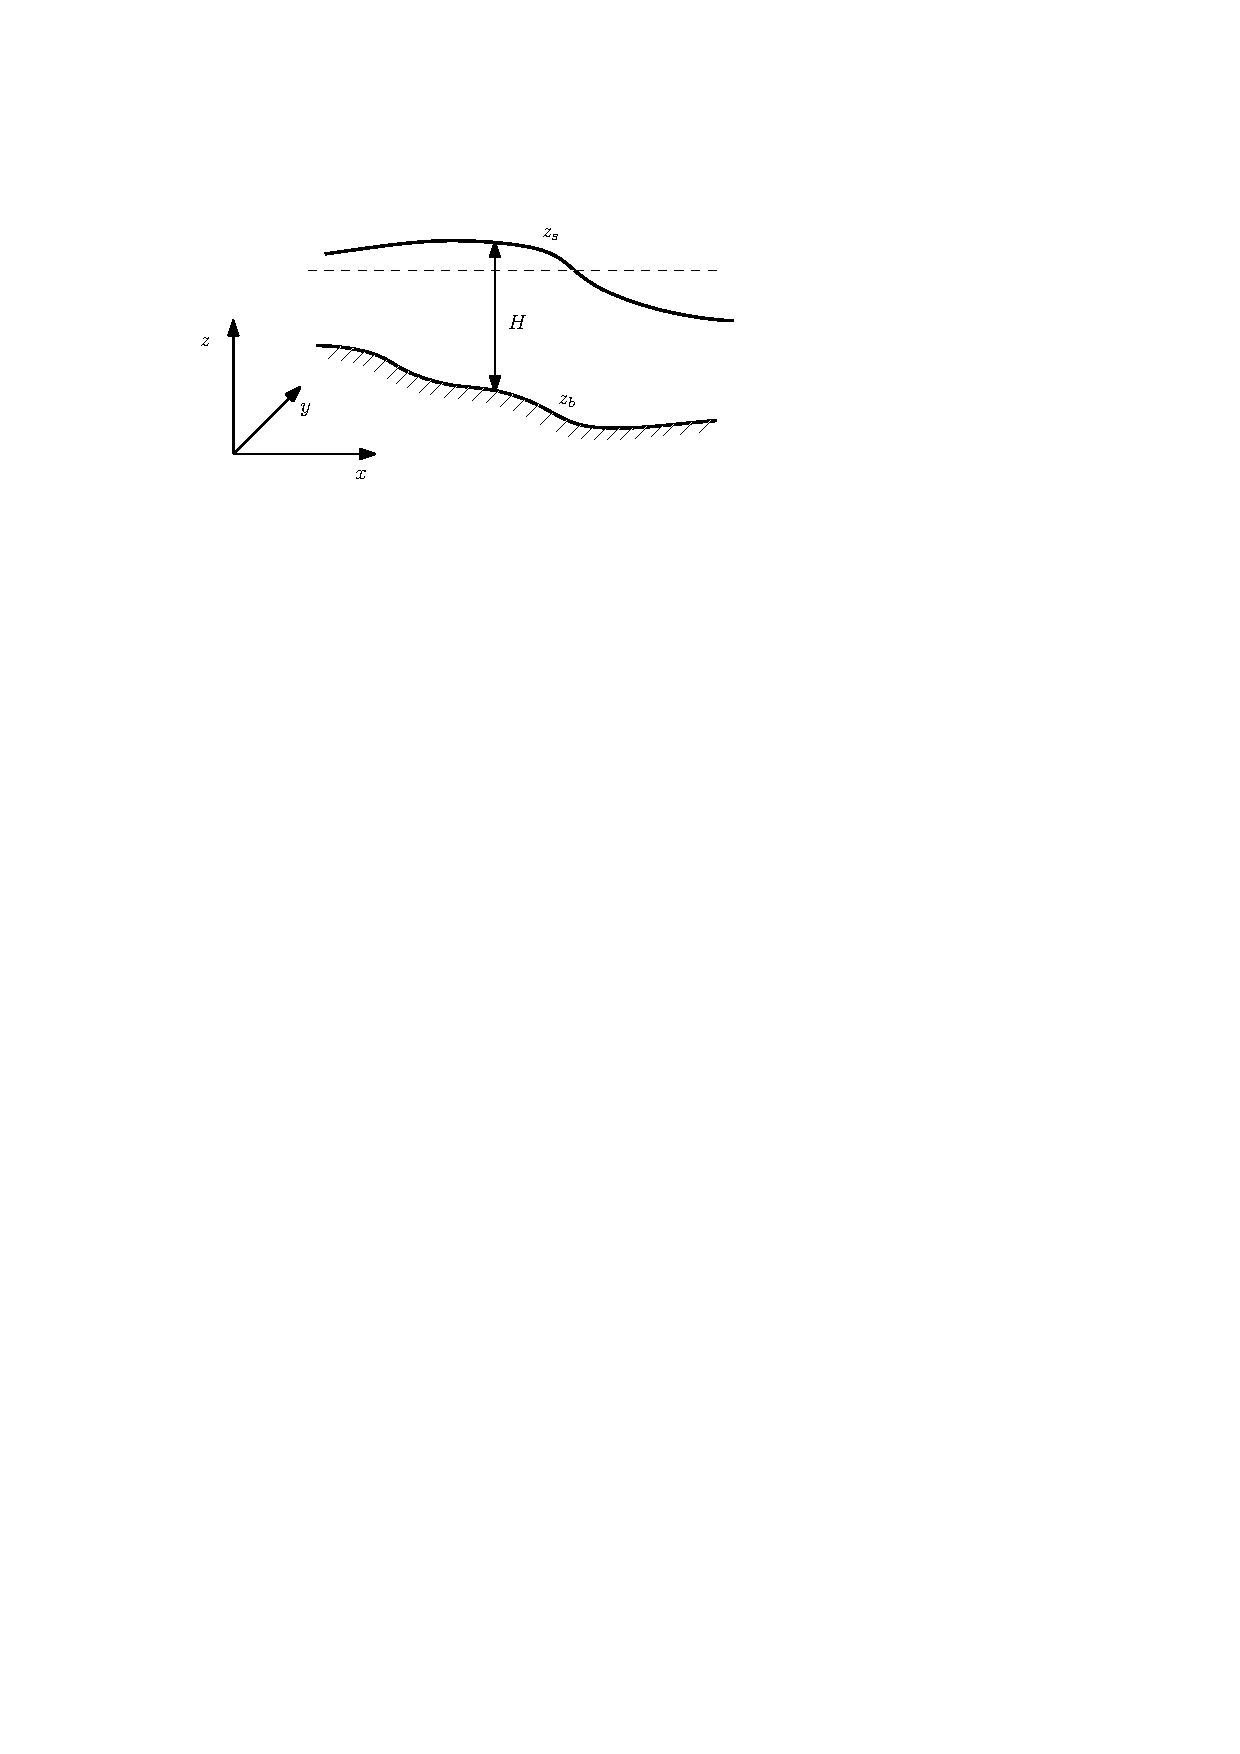
\includegraphics{CGe2DSweDepth.pdf}
  \caption{水位基准示意图}
  \label{FgCGe_2DSwe_depth}
\end{figure}

(2)定义沿水深平均流速$U$和$V$
\begin{equation}
  U
  =
  \frac{1}{H}
  \int_{z_{b}}^{ z_{s}}\!\overline{u}\mathrm{d}z
  \quad
  \quad
  V
  =
  \frac{1}{H}
  \int_{z_{b}}^{ z_{s}}\!\overline{v}\mathrm{d}z
\end{equation}
%式中,下标$i$取1,2和3分别对应$x$,$y$和$z$方向的速度分量。

(3)莱布尼兹公式
\begin{equation}
  \frac{\partial}{\partial x_{i}}
  \int_{a}^{b}\!f\mathrm{d}z
  =
  \int_{a}^{b}\!
  \frac{\partial f}{\partial x_{i}}\mathrm{d}z
  +
  \left.
  f
  \right|_{b}\frac{\partial b}{\partial x_{i}}
  -
  \left.f\right|_{a}\frac{\partial a}{\partial x_{i}}
  \label{EqCGeLeibnizLaw}
\end{equation}
式中,$x_{i}=x$,$y$,$t$。$a$、$b$和$f$都是$x_{i}$的函数。

(4)自由表面及河床底部运动学条件为:
\begin{equation}
  \left.\overline{w}\right|_{z_{s}}
  =
  \frac{D z_{s}}{Dt}
  =
  \frac{\partial z_{s}}{\partial t}
  +
  \left.\overline{u}\right|_{z_{s}}\frac{\partial z_{s}}{\partial x}
  +
  \left.\overline{v}\right|_{z_{s}}\frac{\partial z_{s}}{\partial y}
  \label{EqCGeSMC}
\end{equation}
\begin{equation}
  \left.\overline{w}\right|_{z_{b}}
  =
  \frac{Dz_{b}}{Dt}
  =
  \frac{\partial z_{b}}{\partial t}
  +
  \left.\overline{u}\right|_{z_{b}}\frac{\partial z_{b}}{\partial x}
  +
  \left.\overline{v}\right|_{z_{b}}\frac{\partial z_{b}}{\partial y}
  \label{EqCGeBMC}
\end{equation}

\subsection{沿水深平均的连续性方程}
采用上述定义和公式对连续性方程\eqref{EqRaeCSimp}沿水深积分平均得:
\begin{equation}
  \int_{z_{b}}^{ z_{s}}\!
  \left(
  \frac{\partial \overline{u}}{\partial x} +
  \frac{\partial \overline{v}}{\partial y} +
  \frac{\partial \overline{w}}{\partial z}
  \right)
  \mathrm{d}z
  =
  0
  \label{EqCGeRaeCE_Int}
\end{equation}
根据式\eqref{EqCGeLeibnizLaw},式\eqref{EqCGeRaeCE_Int}中前两项分别可写成
\begin{equation}
  \int_{z_{b}}^{ z_{s}}\!
  \frac{\partial \overline{u}}{\partial x}
  \mathrm{d}z
  =
  \frac{\partial}{\partial x}
  \int_{z_{b}}^{ z_{s}}\!
  \overline{u}
  \mathrm{d}z
  -
  \left.\overline{u}\right|_{z_{s}}
  \frac{\partial z_{s}}{\partial x}
  +
  \left.\overline{u}\right|_{z_{b}}
  \frac{\partial z_{b}}{\partial x}
  \label{EqCGeRaeCE_Int_x}
\end{equation}
\begin{equation}
  \int_{z_{b}}^{ z_{s}}\!
  \frac{\partial \overline{v}}{\partial y}
  \mathrm{d}z
  =
  \frac{\partial}{\partial y}
  \int_{z_{b}}^{ z_{s}}\!
  \overline{v}
  \mathrm{d}z
  -
  \left.\overline{v}\right|_{z_{s}}
  \frac{\partial z_{s}}{\partial y}
  +
  \left.\overline{v}\right|_{z_{b}}
  \frac{\partial z_{b}}{\partial y}
  \label{EqCGeRaeCE_Int_y}
\end{equation}
式\eqref{EqCGeRaeCE_Int}中最后一项
\begin{equation}
  \int_{z_{b}}^{ z_{s}}\!
  \frac{\partial \overline{w}}{\partial z}
  \mathrm{d}z
  =
  \left.\overline{w}\right|_{z_{s}}
  -
  \left.\overline{w}\right|_{z_{b}}
  \label{EqCGeRaeCE_Int_z}
\end{equation}
将式\eqref{EqCGeRaeCE_Int_x},\eqref{EqCGeRaeCE_Int_y}和\eqref{EqCGeRaeCE_Int_z}
代入\eqref{EqCGeRaeCE_Int},并利用自由表面及河床底部运动学条件式\eqref{EqCGeSMC}
和\eqref{EqCGeBMC},可得
\begin{equation*}
  \begin{aligned}
    &\int_{z_{b}}^{ z_{s}}\!
    \left(
    \frac{\partial \overline{u}}{\partial x} +
    \frac{\partial \overline{v}}{\partial y} +
    \frac{\partial \overline{w}}{\partial z}
    \right)
    \mathrm{d}z
    \\
    =&
    \frac{\partial}{\partial x}
    \int_{z_{b}}^{ z_{s}}\!
    \overline{u}
    \mathrm{d}z
    -
    \left.\overline{u}\right|_{z_{s}}
    \frac{\partial z_{s}}{\partial z}
    +
    \left.\overline{u}\right|_{z_{b}}
    \frac{\partial z_{b}}{\partial z}
    + \\
    &
    \frac{\partial}{\partial y}
    \int_{z_{b}}^{ z_{s}}\!
    \overline{v}
    \mathrm{d}z
    -
    \left.\overline{v}\right|_{z_{s}}
    \frac{\partial z_{s}}{\partial z}
    +
    \left.\overline{v}\right|_{z_{b}}
    \frac{\partial z_{b}}{\partial z}
    + \\
    &
    \left.\overline{w}\right|_{z_{s}}
    -
    \left.\overline{w}\right|_{z_{b}}
    \\
    =&
    \frac{\partial HU}{\partial x} +
    \frac{\partial HV}{\partial x} +
    \frac{\partial  z_{s}}{\partial t} -
    \frac{\partial z_{b}}{\partial t}
    =
    0
  \end{aligned}
\end{equation*}
最后得
\begin{equation}
  \frac{\partial H}{\partial t} +
  \frac{\partial HU}{\partial x} +
  \frac{\partial HV}{\partial y}
  =
  0
\end{equation}
也可以写成
\begin{equation}
  \frac{\partial H}{\partial t} +
  \nabla\cdot(H\mathbf{U})
  =
  0
\end{equation}

\subsection{沿水深平均的运动方程}
以$x$方向为例,式\eqref{EqRaeMexSimp}沿水深积分为
\begin{equation}
  \int_{z_{b}}^{ z_{s}}\!
  \left[
    \frac{\partial \overline{u}}{\partial t} +
    \frac{\partial (\widebar{u}\widebar{u})}{\partial x} +
    \frac{\partial (\widebar{u}\widebar{v})}{\partial y} +
    \frac{\partial (\widebar{u}\widebar{w})}{\partial z} +
    \frac{1}{\rho}\frac{\partial \overline{p}}{\partial x} -
    \nu_{t}
    \left(
    \frac{\partial^{2} \overline{u}}{\partial x^{2}} +
    \frac{\partial^{2} \overline{u}}{\partial y^{2}} +
    \frac{\partial^{2} \overline{u}}{\partial z^{2}}
    \right)
  \right]
  \mathrm{d}z
  =
  0
  \label{EqCGeMex_Int}
\end{equation}
式\eqref{EqCGeMex_Int}中包含了非恒定流项积分、对流项积分、压力项积分和阻力项积分
。接下来分项讨论。

(1)非恒定流项积分
\begin{equation}
  \begin{aligned}
    &
    \int_{z_{b}}^{ z_{s}}\!
    \frac{\partial \overline{u}}{\partial t}
    \mathrm{d}z
    =
    \frac{\partial}{\partial t}
    \int_{z_{b}}^{ z_{s}}\!
    \overline{u}
    \mathrm{d}z
    -
    \left.\overline{u}\right|_{z_{s}}\frac{\partial  z_{s}}{\partial t}
    +
    \left.\overline{u}\right|_{z_{b}}\frac{\partial z_{b}}{\partial t}
    \\
    =&
    \frac{\partial HU}{\partial t}
    -
    \left.\overline{u}\right|_{z_{s}}\frac{\partial  z_{s}}{\partial t}
    +
    \left.\overline{u}\right|_{z_{b}}\frac{\partial z_{b}}{\partial t}
  \end{aligned}
  \label{EqCGe_Mex_US_Int}
\end{equation}

(2)对流项积分

首先将时均流速按照式\eqref{EqCGe_VelDecompse}进行分解
\begin{equation}
  \begin{aligned}
    \overline{u}
    =
    U+\Delta\overline{u}
    \\
    \overline{v}
    =
    V+\Delta\overline{v}
  \end{aligned}
  \label{EqCGe_VelDecompse}
\end{equation}
式中,$\Delta\overline{u}$和$\Delta\overline{v}$分别为$x$和$y$的时均流速与
垂线平均流速的差值。

对流项中第一项的积分
\begin{equation}
  \int_{z_{b}}^{ z_{s}}\!
  \frac{\partial \widebar{u}\widebar{u}}{\partial x}
  \mathrm{d}z
  =
  \frac{\partial}{\partial x}
  \int_{z_{b}}^{ z_{s}}\!
  \widebar{u}\widebar{u}
  \mathrm{d}z
  -
  \left.\widebar{u}\widebar{u}\right|_{z_{s}}\frac{\partial  z_{s}}{\partial x}
  +
  \left.\widebar{u}\widebar{u}\right|_{z_{b}}\frac{\partial z_{b}}{\partial x}
  \label{EqCGe_CT_1st}
\end{equation}
式中
\begin{equation*}
  \begin{aligned}
    \int_{z_{b}}^{ z_{s}}\!
    \widebar{u}\widebar{u}
    \mathrm{d}z
    &=
    \int_{z_{b}}^{ z_{s}}\!
    (U+\Delta\overline{u})(U+\Delta\overline{u})
    \mathrm{d}z
    \\
    &=
    \int_{z_{b}}^{ z_{s}}\!
    (UU+2U\Delta\overline{u}+\Delta\overline{u}\Delta\overline{u})
    \mathrm{d}z
    \\
    &=
    HUU
    +
    \int_{z_{b}}^{ z_{s}}\!
    \Delta\overline{u}\Delta\overline{u}
    \mathrm{d}z
    \\
    &=
    \beta_{xx}HUU
  \end{aligned}
\end{equation*}
其中
\begin{equation}
  \beta_{xx}
  =
  1 +
  \frac
  {
    \int_{z_{b}}^{ z_{s}}\!
    \Delta\overline{U}\Delta\overline{U}
    \mathrm{d}z
  }
  {HUU}
\end{equation}
是由于流速沿垂线分布不均匀而引入的修正系数,类似于水力学中的动量修正系数。
$\beta_{xx}$的取值一般在1.02与1.05之间,可近似取为1.0。因此
\begin{equation}
  \int_{z_{b}}^{ z_{s}}\!
  \frac{\partial \widebar{u}\widebar{u}}{\partial x}
  \mathrm{d}z
  =
  \frac{\partial HUU}{\partial x}
  -
  \left.\widebar{u}\widebar{u}\right|_{z_{s}}\frac{\partial  z_{s}}{\partial x}
  +
  \left.\widebar{u}\widebar{u}\right|_{z_{b}}\frac{\partial z_{b}}{\partial x}
\end{equation}

同理,对流项的第二项可写为
\begin{equation}
  \int_{z_{b}}^{ z_{s}}\!
  \frac{\partial \widebar{u}\widebar{v}}{\partial y}
  \mathrm{d}z
  =
  \frac{\partial HUV}{\partial x}
  -
  \left.\widebar{u}\widebar{v}\right|_{z_{s}}\frac{\partial  z_{s}}{\partial y}
  +
  \left.\widebar{u}\widebar{v}\right|_{z_{b}}\frac{\partial z_{b}}{\partial y}
\end{equation}
对流项的第三项
\begin{equation}
  \int_{z_{b}}^{ z_{s}}\!
  \frac{\partial \widebar{u}\widebar{w}}{\partial z}
  \mathrm{d}z
  =
  \left.\widebar{u}\widebar{w}\right|_{z_{s}}
  -
  \left.\widebar{u}\widebar{w}\right|_{z_{b}}
\end{equation}

将非恒定流项和对流项积分相加,并利用自由表面和河床底部运动学条件可得:
\begin{equation}
  \int_{z_{b}}^{ z_{s}}\!
  \left[
    \frac{\partial \overline{u}}{\partial t} +
    \frac{\partial (\widebar{u}\widebar{u})}{\partial x} +
    \frac{\partial (\widebar{u}\widebar{v})}{\partial y} +
    \frac{\partial (\widebar{u}\widebar{w})}{\partial z}
  \right]
  \mathrm{d}z
  =
  \frac{\partial HU}{\partial t}
  +
  \frac{\partial HUU}{\partial x}
  +
  \frac{\partial HUV}{\partial y}
\end{equation}

(3)压力项积分
\begin{equation}
  \begin{aligned}
    \int_{z_{b}}^{ z_{s}}\!
    \frac{\partial \overline{p}}{\partial x}
    \mathrm{d}z
    &=
    \frac{\partial}{\partial x}
    \int_{z_{b}}^{ z_{s}}\!
    \overline{p}
    \mathrm{d}z
    -
    \left.\overline{p}\right|_{z_{s}}\frac{\partial  z_{s}}{\partial x}
    +
    \left.\overline{p}\right|_{z_{b}}\frac{\partial z_{b}}{\partial x}
    \\
    &=
    \frac{\partial}{\partial x}
    \int_{z_{b}}^{ z_{s}}\!
    \rho g( z_{s}-z)
    \mathrm{d}z
    -
    \left.\rho g( z_{s}-z)\right|_{z_{s}}\frac{\partial  z_{s}}{\partial x}
    +
    \left.\rho g( z_{s}-z)\right|_{z_{b}}\frac{\partial z_{b}}{\partial x}
    \\
    &=
    \rho gH\frac{\partial H}{\partial x}
    +
    \rho gH\frac{\partial z_{b}}{\partial x}
    =
    \rho gH\frac{\partial  z_{s}}{\partial x}
  \end{aligned}
\end{equation}

(4)阻力项积分
\begin{equation}
  \begin{aligned}
    &\int_{z_{b}}^{ z_{s}}\!
    \frac{\partial^{2} \overline{u}}{\partial x^{2}}
    \mathrm{d}z
    =
    \int_{z_{b}}^{ z_{s}}\!
    \frac{\partial}{\partial x}
    \left(\frac{\partial \overline{u}}{\partial x}\right)
    \mathrm{d}z
    =
    \frac{\partial}{\partial x}
    \int_{z_{b}}^{ z_{s}}\!
    \frac{\partial \overline{u}}{\partial x}
    \mathrm{d}z
    -
    \left.\frac{\partial \overline{u}}{\partial x}\right|_{z_{s}}\frac{\partial  z_{s}}{\partial x}
    +
    \left.\frac{\partial \overline{u}}{\partial x}\right|_{z_{b}}\frac{\partial z_{b}}{\partial x}
    \\
    =&
    \frac{\partial}{\partial x}
    \left(
    \frac{\partial}{\partial x}
    \int_{z_{b}}^{ z_{s}}\!
    \overline{u}
    \mathrm{d}z
    -
    \left.\overline{u}\right|_{z_{s}}\frac{\partial  z_{s}}{\partial x}
    +
    \left.\overline{u}\right|_{z_{b}}\frac{\partial z_{b}}{\partial x}
    \right)
    -
    \left.\frac{\partial \overline{u}}{\partial x}\right|_{z_{s}}\frac{\partial  z_{s}}{\partial x}
    +
    \left.\frac{\partial \overline{u}}{\partial x}\right|_{z_{b}}\frac{\partial z_{b}}{\partial x}
    \\
    =&
    \frac{\partial^{2} HU}{\partial x^{2}} +
    \frac{\partial}{\partial x}
    \left(
    -
    \left.\overline{u}\right|_{z_{s}}\frac{\partial  z_{s}}{\partial x}
    +
    \left.\overline{u}\right|_{z_{b}}\frac{\partial z_{b}}{\partial x}
    \right)
    -
    \left.\frac{\partial \overline{u}}{\partial x}\right|_{z_{s}}\frac{\partial  z_{s}}{\partial x}
    +
    \left.\frac{\partial \overline{u}}{\partial x}\right|_{z_{b}}\frac{\partial z_{b}}{\partial x}
  \end{aligned}
  \label{EqCGe_Shear_1}
\end{equation}

类似地
\begin{equation}
  \int_{z_{b}}^{ z_{s}}\!
  \frac{\partial^{2} \overline{u}}{\partial y^{2}}
  \mathrm{d}z
  =
  \frac{\partial^{2} HU}{\partial y^{2}} +
  \frac{\partial}{\partial y}
  \left(
  -
  \left.\overline{u}\right|_{z_{s}}\frac{\partial  z_{s}}{\partial y}
  +
  \left.\overline{u}\right|_{z_{b}}\frac{\partial z_{b}}{\partial y}
  \right)
  -
  \left.\frac{\partial \overline{u}}{\partial y}\right|_{z_{s}}\frac{\partial  z_{s}}{\partial y}
  +
  \left.\frac{\partial \overline{u}}{\partial y}\right|_{z_{b}}\frac{\partial z_{b}}{\partial y}
  \label{EqCGe_Shear_2}
\end{equation}
\begin{equation}
  \int_{z_{b}}^{ z_{s}}\!
  \frac{\partial^{2} \overline{u}}{\partial z^{2}}
  \mathrm{d}z
  =
  \left.\frac{\partial \overline{u}}{\partial z}\right|_{z_{s}}
  -
  \left.\frac{\partial \overline{u}}{\partial z}\right|_{z_{b}}
  \label{EqCGe_Shear_3}
\end{equation}
将式\eqref{EqCGe_Shear_1}至\eqref{EqCGe_Shear_3}相加,得
\begin{equation}
  \begin{aligned}
    &\int_{z_{b}}^{ z_{s}}\!
    \nu_{t}
    \left(
    \frac{\partial^{2} \overline{u}}{\partial x^{2}} +
    \frac{\partial^{2} \overline{u}}{\partial y^{2}} +
    \frac{\partial^{2} \overline{u}}{\partial z^{2}}
    \right)
    \mathrm{d}z =\\
    &
    \nu_{t}
    \left(
    \frac{\partial^{2} HU}{\partial x^{2}} +
    \frac{\partial^{2} HU}{\partial y^{2}}
    \right)
    \\
    -&\nu_{t}
    \left[
      \frac{\partial}{\partial x}
      \left(
      \frac{\partial  z_{s}}{\partial x}
      \left.\overline{u}\right|_{z_{s}}
      \right)
      +
      \frac{\partial}{\partial y}
      \left(
      \frac{\partial  z_{s}}{\partial y}
      \left.\overline{u}\right|_{z_{s}}
      \right)
      +
      \left.\frac{\partial \overline{u}}{\partial x}\right|_{z_{s}}
      \frac{\partial  z_{s}}{\partial x}
      +
      \left.\frac{\partial \overline{u}}{\partial y}\right|_{z_{s}}
      \frac{\partial  z_{s}}{\partial y}
      -
      \left.\frac{\partial \overline{u}}{\partial z}\right|_{z_{s}}
    \right]
    \\
    +&\nu_{t}
    \left[
      \frac{\partial}{\partial x}
      \left(
      \frac{\partial z_{b}}{\partial x}
      \left.\overline{u}\right|_{z_{b}}
      \right)
      +
      \frac{\partial}{\partial y}
      \left(
      \frac{\partial z_{b}}{\partial y}
      \left.\overline{u}\right|_{z_{b}}
      \right)
      +
      \left.\frac{\partial \overline{u}}{\partial x}\right|_{z_{b}}
      \frac{\partial z_{b}}{\partial x}
      +
      \left.\frac{\partial \overline{u}}{\partial y}\right|_{z_{b}}
      \frac{\partial z_{b}}{\partial y}
      -
      \left.\frac{\partial \overline{u}}{\partial z}\right|_{z_{b}}
    \right]
  \end{aligned}
  \label{EqCGe_Shear_Total}
\end{equation}
式\eqref{EqCGe_Shear_Total}中右边后两项分别为由底部床面阻力和自由表面风阻力引起
的阻力项,通常可以式\eqref{EqCGe_Shear}表示:
\begin{equation}
  g\frac{n^{2}U\sqrt{U^{2}+V^{2}}}{H^{1/3}}
  -
  C_{w}\frac{\rho_{a}}{\rho}\omega^{2}\cos\beta
  \label{EqCGe_Shear}
\end{equation}
式中,$C_{w}$为无因次风应力系数,$\rho_{a}$为空气密度,$\omega$为风速,$\beta$为
风向与$x$方向的夹角。最后,$x$方向的运动方程为
\begin{equation}
  \begin{aligned}
    \frac{\partial HU}{\partial t} +
    &\frac{\partial HUU}{\partial x} +
    \frac{\partial HUV}{\partial y}
    =\\
    &-gH\frac{\partial  z_{s}}{\partial x}
    -g\frac{n^{2}U\sqrt{U^{2}+V^{2}}}{H^{1/3}}
    +
    \nu_{t}\left(
    \frac{\partial^{2}HU}{\partial x^{2}}+
    \frac{\partial^{2}HU}{\partial y^{2}}
    \right)
    +C_{w}\frac{\rho_{a}}{\rho}\omega^{2}\cos\beta
  \end{aligned}
  \label{EqCGe_Me_x}
\end{equation}
同理可得,$y$方向运动方程为
\begin{equation}
  \begin{aligned}
    \frac{\partial HV}{\partial t} +
    &\frac{\partial HUV}{\partial x} +
    \frac{\partial HVV}{\partial y}
    =\\
    &-gH\frac{\partial  z_{s}}{\partial y}
    -g\frac{n^{2}V\sqrt{U^{2}+V^{2}}}{H^{1/3}}
    +
    \nu_{t}\left(
    \frac{\partial^{2}HV}{\partial x^{2}}+
    \frac{\partial^{2}HV}{\partial y^{2}}
    \right)
    +C_{w}\frac{\rho_{a}}{\rho}\omega^{2}\sin\beta
  \end{aligned}
  \label{EqCGe_Me_y}
\end{equation}

当自由表面风应力影响较小时,风应力项可以忽略。此外,当模拟区域尺度较大,还要考虑
地球自转的影响,可在方程\eqref{EqCGe_Me_x}和\eqref{EqCGe_Me_y}右边分别加入科氏力。
\begin{equation}
  \begin{aligned}
    f_x = 2\omega\sin\varphi U
    \\
    f_y = 2\omega\sin\varphi V
  \end{aligned}
\end{equation}
式中,$\omega$为地球自转角速度,$\varphi$为模拟区域所处纬度。

根据推导过程中所采用的假定条件,在使用二维浅水方程时应注意以下问题:
\begin{enumerate}
  \item 方程推导中引用了牛顿流体所满足的本构关系式,因此上述方程只适用于牛顿流体
    ,对类似高含沙水流的非牛顿流体不适用。
  \item 方程推导中对流体做了均质不可压的假设,因此上述方程只能在含沙量较小的情况下近似使
    用,当含沙量较大时,应考虑密度变化的影响。
  \item 在垂向积分过程中,略去流速等水力参数沿垂直方向的变化,并假定沿水深方向的动水压强
    分布符合静水压强分布。因此所研究问题的水平尺度应远大于垂向尺度,流速等水力参数沿
    垂直方向的变化较之沿水平方向的变化要小得多。
\end{enumerate}

\subsection{二维平面浅水方程不同形式}
忽略风应力和科氏力的二维平面浅水方程为
\begin{equation}
  \begin{gathered}
    \frac{\partial H}{\partial t} +
    \frac{\partial HU}{\partial x} +
    \frac{\partial HV}{\partial y}
    =
    0
    \\
    \frac{\partial HU}{\partial t} +
    \frac{\partial HUU}{\partial x} +
    \frac{\partial HUV}{\partial y}
    =
    -gH\frac{\partial  z_{s}}{\partial x}
    -g\frac{n^{2}U\sqrt{U^{2}+V^{2}}}{H^{1/3}}
    +
    \nu_{t}\left(
    \frac{\partial^{2}HU}{\partial x^{2}}+
    \frac{\partial^{2}HU}{\partial y^{2}}
    \right)
    \\
    \frac{\partial HV}{\partial t} +
    \frac{\partial HUV}{\partial x} +
    \frac{\partial HVV}{\partial y}
    =
    -gH\frac{\partial  z_{s}}{\partial y}
    -g\frac{n^{2}V\sqrt{U^{2}+V^{2}}}{H^{1/3}}
    +
    \nu_{t}\left(
    \frac{\partial^{2}HV}{\partial x^{2}}+
    \frac{\partial^{2}HV}{\partial y^{2}}
    \right)
  \end{gathered}
\end{equation}

当床面阻力占主导作用时,还可进一步忽略紊动阻力项。
\begin{equation}
  \begin{gathered}
    \frac{\partial H}{\partial t} +
    \frac{\partial HU}{\partial x} +
    \frac{\partial HV}{\partial y}
    =
    0
    \\
    \frac{\partial HU}{\partial t} +
    \frac{\partial (HUU+gH^{2}/2)}{\partial x} +
    \frac{\partial HUV}{\partial y}
    =
    -gH\frac{\partial z_{b}}{\partial x}
    -g\frac{n^{2}U\sqrt{U^{2}+V^{2}}}{H^{1/3}}
    \\
    \frac{\partial HV}{\partial t} +
    \frac{\partial HUV}{\partial x} +
    \frac{\partial (HVV+gH^{2}/2)}{\partial y}
    =
    -gH\frac{\partial z_{b}}{\partial y}
    -g\frac{n^{2}V\sqrt{U^{2}+V^{2}}}{H^{1/3}}
  \end{gathered}
\end{equation}

此外,为了书写的简化,用$h$替代$H$,$u$替代$U$,$v$替代$V$,定义$x$和$y$
方向的流量分别为$q_{x}=hu$和$q_{y}=hv$,上式可写成
\begin{equation}
  \begin{gathered}
    \frac{\partial h}{\partial t} +
    \frac{\partial q_{x}}{\partial x} +
    \frac{\partial q_{y}}{\partial y}
    =
    0
    \\
    \frac{\partial q_{x}}{\partial t} +
    \frac{\partial (uq_{x}+gh^{2}/2)}{\partial x} +
    \frac{\partial vq_{y}}{\partial y}
    =
    -gh\frac{\partial z_{b}}{\partial x}
    -g\frac{n^{2}u\sqrt{u^{2}+v^{2}}}{h^{1/3}}
    \\
    \frac{\partial q_{y}}{\partial t} +
    \frac{\partial uq_{y}}{\partial x} +
    \frac{\partial (vq_{y}+gh^{2}/2)}{\partial y}
    =
    -gh\frac{\partial z_{b}}{\partial y}
    -g\frac{n^{2}v\sqrt{u^{2}+v^{2}}}{h^{1/3}}
  \end{gathered}
\end{equation}
上式的向量形式为:
\begin{equation}
  \frac{\partial \mathbf{U}}{\partial t} +
  \frac{\partial \mathbf{F}}{\partial x} +
  \frac{\partial \mathbf{G}}{\partial y}
  =
  \mathbf{S}
\end{equation}
%或
%\begin{equation}
%\frac{\partial \mathbf{q}}{\partial t} +
%\nabla\cdot(\mathbf{F}) =
%\mathbf{S}
%\end{equation}
其中,$\mathbf{U}$为守恒变量向量,$\mathbf{F}$和$\mathbf{G}$分别为$x$和$y$方向的
通量向量,$\mathbf{S}$为河床底坡和阻力源项向量。这些向
量的具体元素为:
\begin{equation}
  \mathbf{U} =
  \begin{bmatrix}
    h \\
    hu \\
    hv \\
  \end{bmatrix}
  ,
  \mathbf{F} =
  \begin{bmatrix}
    hu \\
    hu^{2} + \frac{1}{2}gh^{2} \\
    huv \\
  \end{bmatrix}
  ,
  \mathbf{G} =
  \begin{bmatrix}
    hv \\
    huv \\
    hv^{2} + \frac{1}{2}gh^{2} \\
  \end{bmatrix}
  ,
  \mathbf{S} =
  \begin{bmatrix}
    0 \\
    gh({s_{0}}_{x} - {s_{f}}_{x})\\
    gh({s_{0}}_{y} - {s_{f}}_{y})\\
  \end{bmatrix}
\end{equation}
其中:
\begin{equation}
  {s_{0}}_{x} = - \frac{\partial z_{b}}{\partial x}, 
  {s_{0}}_{y} = - \frac{\partial z_{b}}{\partial y}, 
  {s_{f}}_{x} = - \frac{n^{2}u\sqrt{u^2+v^2}}{h^{4/3}}, 
  {s_{f}}_{y} = - \frac{n^{2}v\sqrt{u^2+v^2}}{h^{4/3}} 
\end{equation}


\section{一维非恒定流基本控制方程}
\subsection{一维连续性方程}
如图\ref{FgCGe_1DSwe}所示,在明槽非恒定流中,沿水流流动方向取长为$\mathrm{d}x$的微小
流段。流段进口1-1断面流量为$Q$,在$\Delta t$时段内,从1-1断面进入流段的液体
质量为$\rho Q\Delta t$。流段出口2-2断面流量为$Q+\frac{\partial Q}{\partial
x}\mathrm{d}x$,在$\Delta t$时段内,从2-2断面流出的液体质量为$\rho Q\Delta
t+\rho\frac{\partial Q}{\partial x}\mathrm{d}x\Delta t$。该时段内进出此流段的液体
质量差为$-\rho\frac{\partial Q}{\partial x}\mathrm{d}x\Delta t$。


\begin{figure}[hb]
  \centering
  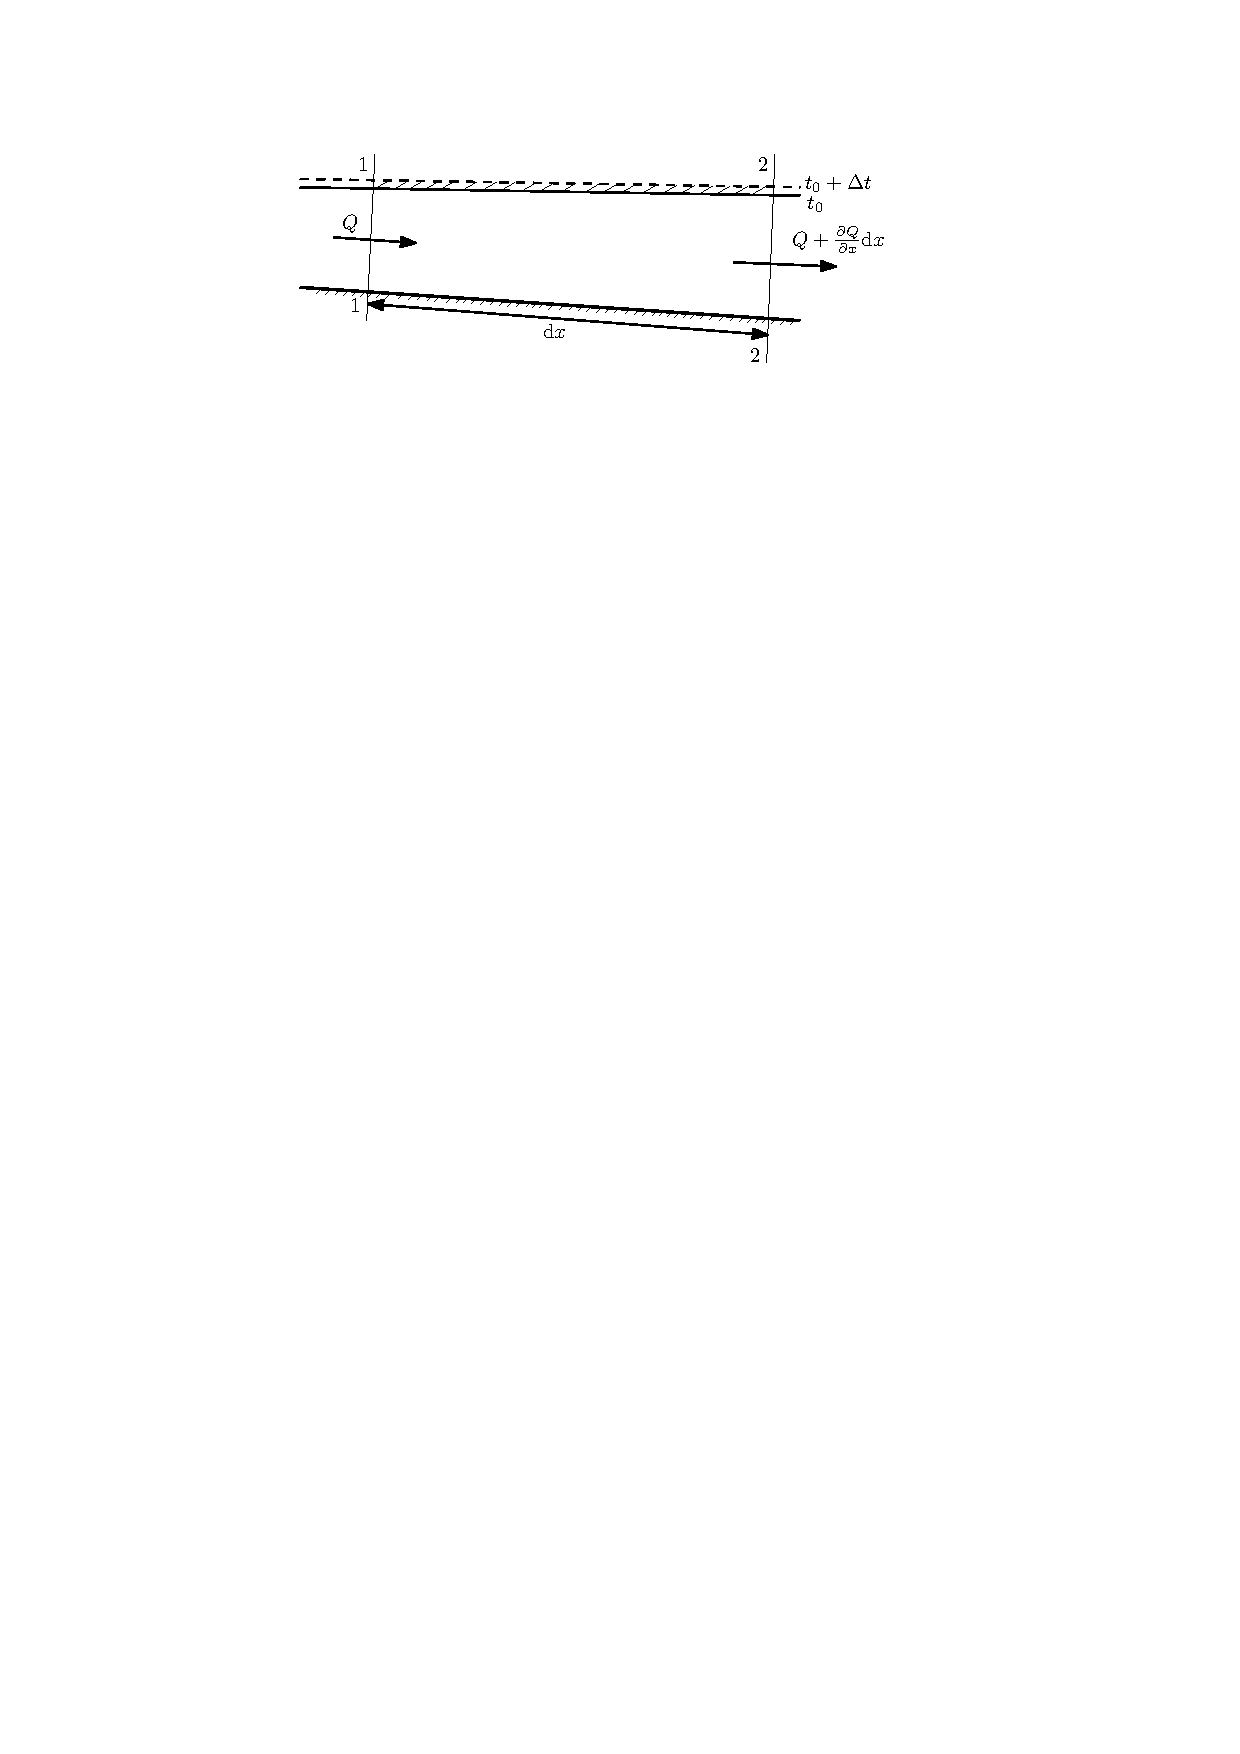
\includegraphics{CGeSW.pdf}
  \caption{一维水流运动示意图}
  \label{FgCGe_1DSwe}
\end{figure}


时段内的质量差表现为流段内的槽蓄量变化。在起始时刻,流段内的槽蓄量为
$\rho\overline{A}\mathrm{d}x$。而经过$\Delta t$时段后,流段内的槽蓄量为
$\rho\left(\overline{A}+\frac{\partial\overline{A}}{\partial t}\Delta
t\right)\mathrm{d}x$。$\Delta t$时段内,流段内的槽蓄量变化量为
$\rho\frac{\partial \overline{A}}{\partial t}\Delta t\mathrm{d}x$。其中
$\overline{A}$为微小流段的平均过水面积。当流段内过水断面面积变化较小时,可直接用
1-1断面段面积$A$来替代$\overline{A}$。

因此,根据质量守恒原理,进出该流段的液体质量差等于流段内槽蓄量改变量,即
\begin{equation*}
  -\rho\frac{\partial Q}{\partial x}\mathrm{d}x\Delta t
  =
  \rho\frac{\partial A}{\partial t}\mathrm{d}x\Delta t
\end{equation*}
化简后得到明槽一维非恒定流连续性方程
\begin{equation}
  \frac{\partial A}{\partial t}
  +
  \frac{\partial Q}{\partial x}
  =
  0
  \label{EqCGe_SVe_Ce}
\end{equation}

如果在该流段内有旁侧入流或出流,且单位长度旁侧入流流量为$q$($q>0$为入流,$q<0$为出流
),考虑旁侧入流得明槽一维非恒定流连续性方程为
\begin{equation}
  \frac{\partial A}{\partial t}
  +
  \frac{\partial Q}{\partial x}
  =
  q
\end{equation}

\subsection{一维运动方程}
设坐标轴$x$方向与水流流动方向一致,根据牛顿第二定律建立运动方程。为分析简单起见
,首先考虑棱柱体明槽(如
图\ref{FgCGe_1DSwe_Force})的情况。

\begin{figure}[htb]
  \centering
  \subfloat[]{\label{FgCGe_1DSwe_Force_a}
  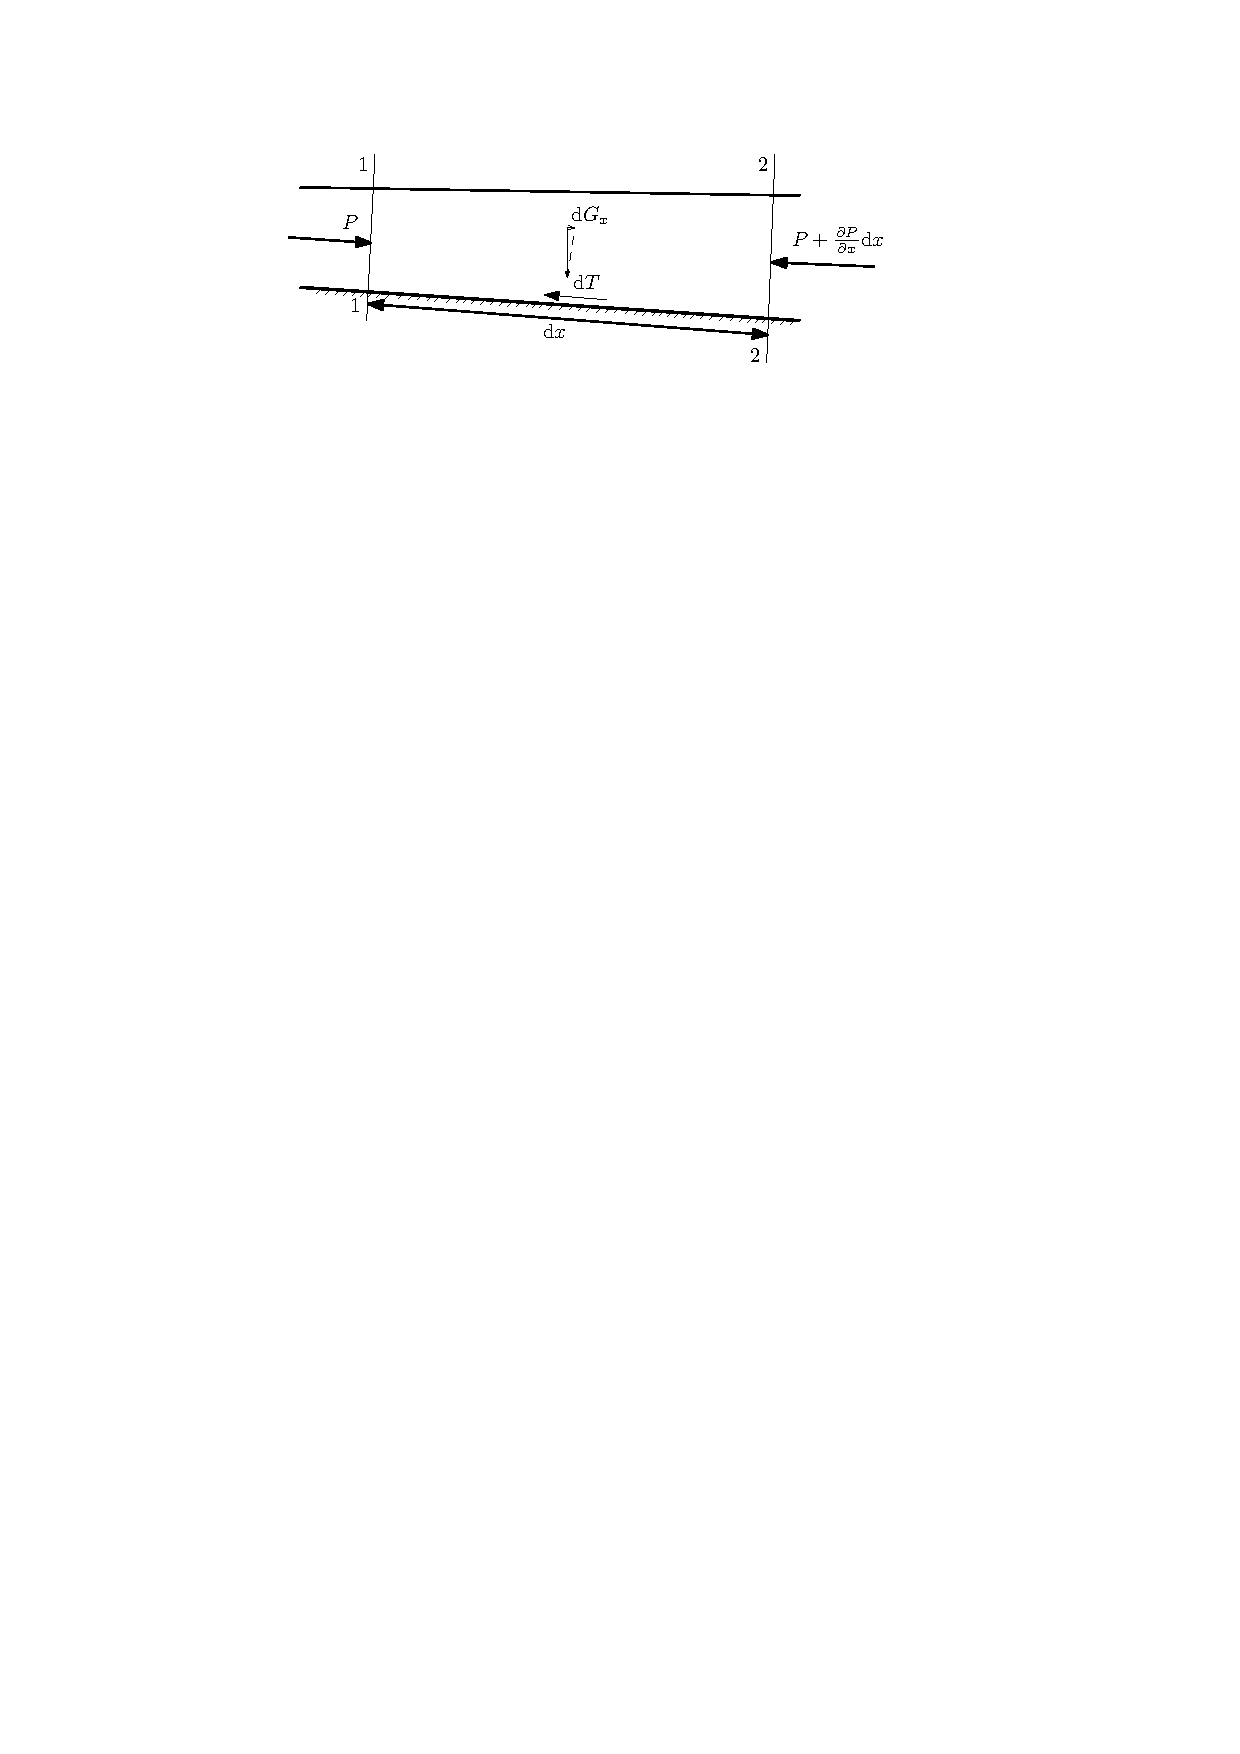
\includegraphics{CGeSW_Force.pdf}
}
\subfloat[]{\label{FgCGe_1DSwe_Force_b}
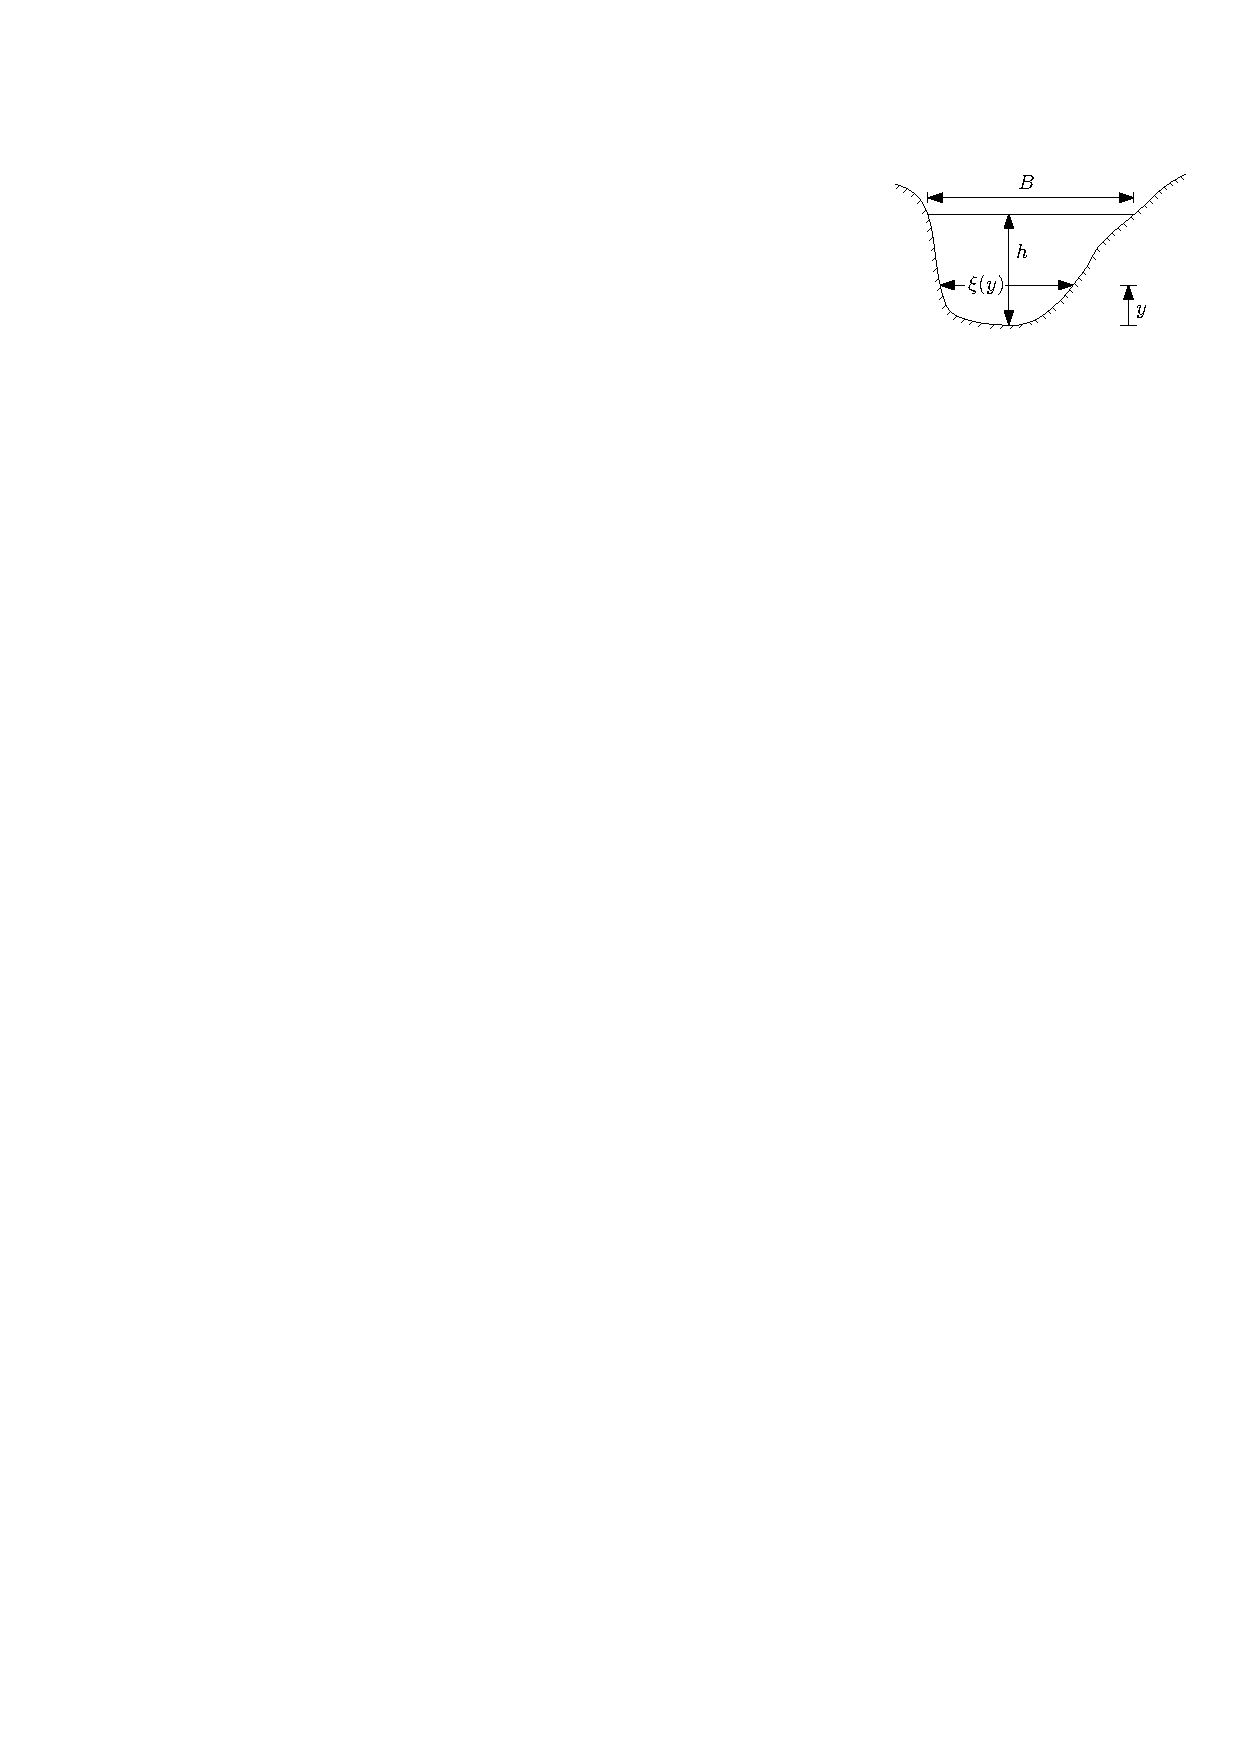
\includegraphics{CGeSW_Pressure.pdf}
}
\caption{一维水流运动示意图}
\label{FgCGe_1DSwe_Force}
\end{figure}


作用在1-1断面的所有外力在$x$方向的分力有:

(1)总动水压力。

设压强分布服从静水压强分布,则作用在1-1断面的水压力
\begin{equation}
  P
  =
  \int_{0}^{h}\! \rho g(h-y)\xi(y)\mathrm{d}y
\end{equation}
式中,$\xi(y)$为过水断面上距渠底$y$处的宽度。
作用于2-2断面的水压力为$P+\frac{\partial P}{\partial x}\mathrm{d}x$。则沿$x$方向
的总动水压力
\begin{equation}
  \begin{aligned}
    \sum P
    =&
    P - \left(P+\frac {\partial P} {\partial x}\mathrm{d}x\right)
    \\
    =&
    -\gamma \mathrm{d}x
    \left[
      \frac{\partial h}{\partial x}
      \int_{0}^{h}\!
      \xi(y)
      \mathrm{d}y
      +
      \int_{0}^{h}\!
      (h-y)
      \frac{\partial \xi(y)}{\partial x}
      \mathrm{d}y
    \right]
  \end{aligned}
  \label{EqCGe_SVe_Me_Pressure}
\end{equation}
因假定明槽为棱柱体明槽,有$\frac{\partial \xi(y)}{\partial x}=0$。则有
\begin{equation}
  \sum P
  =
  -\gamma A\frac{\partial h}{\partial x}\mathrm{d}x
\end{equation}

(2)重力
\begin{equation}
  \mathrm{d}G_{x}
  =
  \mathrm{d}G\sin\alpha
  =
  -\gamma A\mathrm{d}x\frac{\partial z_{b}}{\partial x}
\end{equation}
式中,$\alpha$为坐标轴$x$与水平方向的夹角,$A$为过水断面面积。

(3)侧壁面上的阻力
\begin{equation}
  \mathrm{d}T
  =
  \tau_{0}\chi\mathrm{d}x
  =
  \gamma RJ\chi\mathrm{d}x
  =
  \gamma AJ\mathrm{d}x
\end{equation}
式中,$\chi$为过水断面湿周,$R$为过水断面水力半径,$J$为水力坡度,
$\tau_{0}=\gamma RJ$为侧壁表面平均切应力。

其次,由于流速$U$是$x$和$t$的函数,则水流沿$x$方向的加速度$a_{x}$为
\begin{equation}
  a_{x}
  =
  \frac{\mathrm{d} U}{\mathrm{d} t}
  =
  \frac{\partial U}{\partial t}
  +
  U
  \frac{\partial U}{\partial x}
\end{equation}
微小流段内的水体质量为$\mathrm{d}m=\rho A\mathrm{d}x$。

根据牛顿第二定律,有$\sum F_{x}=\mathrm{d}ma_{x}$,即
\begin{equation}
  -\gamma A\frac{\partial h}{\partial x}\mathrm{d}x
  -\gamma A\frac{\partial z_{b}}{\partial x}\mathrm{d}x
  -\gamma AJ\mathrm{d}x
  =
  \rho A\mathrm{d}x
  \left(
  \frac{\partial U}{\partial t}
  +
  U
  \frac{\partial U}{\partial x}
  \right)
\end{equation}
上式两边同除以$\gamma A\mathrm{d}x$并整理得:
\begin{equation}
  \frac{\partial z}{\partial x}
  +
  \frac{1}{g}
  \frac{\partial U}{\partial t}
  +
  \frac{U}{g}
  \frac{\partial U}{\partial x}
  +
  J
  =
  0
  \label{EqCGe_SVe_Me}
\end{equation}
式\eqref{EqCGe_SVe_Me}即为棱柱体明槽非恒定流运动方程得一般形式。对于非棱柱体明槽
(比如河槽向下游缩窄或展宽),则两岸壁将对微小流段水体作用一附加压力,该附加压力
可表示为
\begin{equation}
  P^{\prime}
  =
  \int_{0}^{h}\!
  \left[
    \rho g(h-y)
    \frac{\partial \xi(y)}{\partial x}
    \mathrm{d}x
  \right]
  \mathrm{d}y
\end{equation}
将附加压力代式\eqref{EqCGe_SVe_Me_Pressure}入中,恰好与该式最后一项抵消。因此对
于非棱柱体明槽,式\eqref{EqCGe_SVe_Me}仍适用。

\subsection{圣维南方程不同形式}
连续性方程\eqref{EqCGe_SVe_Ce}和运动方程\eqref{EqCGe_SVe_Me}构成了描述明槽非恒定
渐变流的圣维南方程组。在实际应用中,为了使用方便,常对式\eqref{EqCGe_SVe_Ce}和
\eqref{EqCGe_SVe_Me}进行改写,得到不同因变量组合的圣维南方程组。

% Todo: 列出下列各式的具体推导过程。

(1)以水位$z$和流量$Q$为因变量的圣维南方程组
\begin{equation}
  \begin{gathered}
    B\frac{\partial z}{\partial t}
    +
    \frac{\partial Q}{\partial x}
    =
    0
    \\
    \frac{\partial Q}{\partial t}
    +
    \frac{2Q}{A}\frac{\partial Q}{\partial x}
    +
    \left[
      gA -
      B
      \left(
      \frac{Q}{A}
      \right)^{2}
    \right]
    \frac{\partial z}{\partial x}
    =
    \left(
    \frac{Q}{A}
    \right)^{2}
    \left.
    \frac{\partial A}{\partial x}
    \right|_{z}
    -
    gA\frac{Q^{2}}{K^{2}}
  \end{gathered}
  \label{EqCGe_SV_zQ}
\end{equation}

(2)以水深$h$和流量$Q$为因变量的圣维南方程组
\begin{equation}
  \begin{gathered}
    B\frac{\partial h}{\partial t}
    +
    \frac{\partial Q}{\partial x}
    =
    0
    \\
    \frac{\partial Q}{\partial t}
    +
    \frac{2Q}{A}\frac{\partial Q}{\partial x}
    +
    \left[
      gA -
      B
      \left(
      \frac{Q}{A}
      \right)^{2}
    \right]
    \frac{\partial h}{\partial x}
    =
    \left(
    \frac{Q}{A}
    \right)^{2}
    \left.
    \frac{\partial A}{\partial x}
    \right|_{h}
    -
    gA\frac{Q^{2}}{K^{2}}
  \end{gathered}
  \label{EqCGe_SV_hQ}
\end{equation}



(3)以水位$z$和流量$U$为因变量的圣维南方程组
\begin{equation}
  \begin{gathered}
    \frac{\partial z}{\partial t}
    +
    U\frac{\partial z}{\partial x}
    +
    \frac{A}{B}\frac{\partial U}{\partial x}
    =
    \frac{1}{B}
    \left(
    q - BiU - U\left.\frac{\partial A}{\partial x}\right|_{z}
    \right)
    \\
    \frac{\partial U}{\partial t}
    +
    U\frac{\partial U}{\partial x}
    +
    g\frac{\partial z}{\partial x}
    =
    -g\frac{U^{2}}{C^{2}R}
  \end{gathered}
  \label{EqCGe_SV_zU}
\end{equation}

(4)以水深$h$和流量$U$为因变量的圣维南方程组
\begin{equation}
  \begin{gathered}
    \frac{\partial h}{\partial t}
    +
    U\frac{\partial h}{\partial x}
    +
    \frac{A}{B}\frac{\partial U}{\partial x}
    =
    \frac{1}{B}
    \left(
    q - U\left.\frac{\partial A}{\partial x}\right|_{h}
    \right)
    \\
    \frac{\partial U}{\partial t}
    +
    U\frac{\partial U}{\partial x}
    +
    g\frac{\partial z}{\partial x}
    =
    g
    \left(
    i-\frac{U^{2}}{C^{2}R}
    \right)
  \end{gathered}
  \label{EqCGe_SV_hU}
\end{equation}

(5)以过水断面
面积$A$和$Q$为因变量的圣维南方程组
\begin{equation}
  \begin{gathered}
    \frac{\partial A}{\partial t}
    +
    \frac{\partial Q}{\partial x}
    =
    0
    \\
    \frac{\partial Q}{\partial t}
    +
    \frac{\partial}{\partial x}\left(\frac{Q^{2}}{A} + gA\frac{\partial h}{\partial x}\right)
    =
    gAi
    -
    gA\frac{n^{2}Q|Q|}{AR^{4/3}}
  \end{gathered}
  \label{EqCGe_SV_AQ_2}
\end{equation}
或
\begin{equation}
  \begin{gathered}
    \frac{\partial A}{\partial t}
    +
    \frac{\partial Q}{\partial x}
    =
    0
    \\
    \frac{\partial Q}{\partial t}
    +
    \frac{\partial}{\partial x}\left(\frac{Q^{2}}{A}+gI\right)
    =
    gAi
    -g\frac{n^{2}|U|}{R^{4/3}}Q
  \end{gathered}
  \label{EqCGe_SV_AQ_1}
\end{equation}
其中, $I = \int_{0}^{h(x,t)}(h-\eta)\frac{\partial A(x, \eta )}{\partial \eta}
\mathrm{d}\eta$。对矩形渠道,\
\begin{equation}
  I = \frac{A^{2 }}{2B}
\end{equation}

该方程组的矩阵形式为
\begin{equation}
\frac{\partial \mathbf{U}}{\partial t} +
\frac{\partial \mathbf{F}}{\partial x} =
\mathbf{G}
\end{equation}

\begin{equation}
  \mathbf{U} =
  \begin{bmatrix}
    A \\
    Q \\
  \end{bmatrix}
  ,
  \mathbf{F} =
  \begin{bmatrix}
    Q \\
    \frac{Q^{2}}{A}+gI \\
  \end{bmatrix}
  ,
  \mathbf{G} =
  \begin{bmatrix}
    0 \\
    gA(i - \frac{n^{2}|Q|Q}{A^{2}R^{4/3 }}) \\
  \end{bmatrix}
\end{equation}

\section{偏微分方程类型和性质}
\subsection{偏微分方程形式}
本章前几节所推导的方程都属于偏微分方程,形式各异。对同一模型建立的控制方程也有多
种不同的形式。在数值计算中,若控制方程的对流项采用散度的形式来表示,这类方程被称
为守恒型的控制方程,否则被称为非恒定形式。

理论上,从微元体角度来看,守恒型微分方程和非守恒型微分方程是等价的,都是同一物理
定律的数学表示。但是,数值计算是对有限大小的计算单元进行的,对有限大小的计算体积
,两种形式的控制方程有不同的特性。守恒型微分方程允许流动参数在计算单元或控制体内
部存在间断;而非守恒型微分方程要求流动参数是可微的。因此,基于守恒型微分方程的数
值方法,可以直接用来计算有间断(如激波)的流场,且不用对间断进行任何特殊处理。这
类数值方法被称为激波捕捉方法。而基于非守恒型为微分方程的数值方法,一般无法正确的
计算有间断的流场。为了处理有间断的流动,这类方法必须与激波装配方法联合使用。简单
来说,激波装配方法是把间断从流场中分离出来,当作流场的边界来处理。

\subsection{控制方程的数学分类及其对数值解的影响}
根据偏微分方程理论,偏微分方程可以被划分成不同的类型,方程的类型决定了定解条件的
提法、解的性质以及数值求解过程。

对于二阶二元的拟线性偏微分方程,其数学上的一般形式为:
\begin{equation}
  a\phi_{xx} + b\phi_{xy} + c\phi_{yy} + d\phi_{x} + e\phi_{y} + f\phi = g(x,y)
\end{equation}
式中,下标$x,y$表示对该自变量的偏导数,系数$a,b,c,d,e,f$是因变量$\phi$及自变量
$x,y$的函数。偏微分方程的分类可用下式进行判别:
\begin{equation}
  b^{2} - 4ac
\end{equation}
\begin{description}
  \item  [双曲型微分方程:] $b^{2}-4ac>0$,过区域内任一点有两条特征线。两条特征
    线交叉通过该点,在该点之前是该点的依赖域,之后是该点的影响域。
  \item [抛物型微分方程:] $b^{2}-4ac=0$,过区域内任一点有一条特征线。过该点的特征
    线将求解区域分成两部分,计算从已知的初值处罚,逐步向前推进,依次获得式和与给
    定边界条件的解。
  \item [椭圆型微分方程:] $b^{2}-4ac<0$,过区域内任一点没有特征线。区域内任一点
    的影响区域是整个求解区域。
\end{description}

\subsection{初始条件与边界条件}
初始条件是所研究现象在过程开始时刻的各个求解变量的空间分布,必须予以给定。需要注
意的是,稳态问题不需要初始条件,但是在求解之前需要对求解变量进行初始化。

边界条件是在求解区域的边界上所求解的变量或其一阶导数随空间及时间的变化规律。需要
注意的是,在固体边界上对速度取无滑移边界条件,即在固体边界上流体的速度等于固体表
面的速度,当固体表面静止时,有:
\begin{equation}
u=v=w=0
\end{equation}
另外,在数值计算中有些边界并不是实际的物理边界,而是计算边界,即根据计算需求而虚
拟划定的边界。这类边界上边界条件如何给定与求解的控制方程和实际物理问题有关。
